%\documentclass{article}
\documentclass[12]{article}
\usepackage{times}
\usepackage{natbib}
%\usepackage{multicol}

\usepackage{color}
\usepackage{subfigure}

\newcommand{\blue}[1]{{\color{blue} #1}}
\newcommand{\red}[1]{{\color{red} #1}}
\newcommand{\green}[1]{{\color{cyan} #1}}

\usepackage{amsmath, amssymb, fullpage, amsthm, array, algorithm2e,graphicx}
%\usepackage[dvips]{graphics}
\newtheorem{thm}{Theorem}[section]
\newtheorem{dfn}{Definition}[section]
\newtheorem{cor}{Corollary}[thm]
\newtheorem{con}{Conjecture}[thm]
%\setlength{\parindent}{0in}   % for no indent

%\topmargin -0.10in   % when making pdf
%\textheight 9.15in  % when making pdf



\begin{document}

% Article top matter
%\title{Where's Waldo : Measuring the quality of a lineup}
%\title{Where's Waldo: Looking closely at a Lineup}
\title{Distance Measures for a Lineup}
\author{Niladri Roy Chowdhury, Dianne Cook, Heike Hofmann, Mahbubul Majumder, Yifan Zhao}
\date{\today}  %\today is replaced with the current date
%\date{}
\maketitle

\begin {abstract} 
Graphics play a crucial role in statistical analysis and data mining. This paper describes developments to assist the use of graphics for making inferential statements. It examines the lineup protocol described in \citet{buja:2009}  and \cite{majumder:2011} developing numerical statistics to measure the quality of the lineup. The null plots play a significant role in determining the ease or difficulty of a lineup. Distance measures are developed that describe how close the true data plot is to the null plots, and how close the null plots are to each other. The distribution of the distance measures are also studied. The effect of null generating mechanism and plot types on the measures are examined. An universal distance measure for any data type is suggested. These measures are evaluated by comparison with choices made by human judges, to decide on the best distance measures to use for particular plot types.

%Statistical graphics play a crucial role in exploratory data analysis, model checking and diagnosis. Until recently there were no formal visual methods in place for determining statistical significance of findings. This changed, when \citep{buja:2009} conceptually introduced two protocols for formal tests of visual findings. In this paper we use the lineup protocol \citep{buja:2009} and take a closer look at the null plots that appear in a lineup along with the true plot. Different distance measures between the null plots and the true plot are calculated. On the basis of these distance measures, a measure of ``closeness'' between the null plots and the true plot is defined. A human subjects experiment is conducted using simulated data to provide controlled conditions. Results suggest that some of the distance measures works better than the others in most situations.
\end {abstract}


%{\color{red} Key Ideas:
% \begin{itemize}
%\item Measure ease of a lineup (? signal strength.)
%\item Distance metric that is universal?
%\item Evaluating distance metrics, incorporating turk study data.
%\end{itemize}}
%\begin{multicols}{2}
%\twocolumn

\section{Introduction} 
There have been major advances in statistical graphics over the years, for example, systems like R \citep{R} provide high quality static graphics, and very recently some access to interactive graphics. But the problem remains that graphics are not widely considered to be a part of inferential statistics. Research by \citet{gelman:2004} and \citet{buja:2009} 
potentially changes this. 

\citep{buja:2009} bridges the gulf between conventional statistical inference and exploratory data analysis. Two protocols are proposed namely the Rorschach and the lineup protocol. The Rorschach protocol helps to understand to understand the extent of randomness while the lineup protocol places a statistical plot firmly in the hypothesis testing framework. The plot of the true data is considered to be a test statistic unlike classical inference where the test statistic is numeric. The test statistic is so chosen that it displays any distinctive pattern, if present in case the null hypothesis is not true. This plot is compared with a set of plots, known as null plots, obtained from the appropriate null distribution consistent with the null hypothesis. The lineup is obtained by placing the true data plot, which is the test statistic, randomly among the obtained null plots. Human subjects are asked to identify the plot with most distinct feature(s). The success of human subjects in identifying the true data plot is regarded as evidence against the null hypothesis and the null hypothesis is rejected. 

The lineup protocol was formally tested by \cite{majumder:2011}. The paper provides a head-to-head comparison between the lineup protocol and equivalent conventional test. The testing is done using human subjects from Amazon's Mechanical Turk (\cite{turk}) using simulation to provide controlled conditions for assessing lineups. The results suggest that the visual inference is comparable to conventional tests in a controlled setting of simulation study. The power of a visual test increases with the number of observers, which interestingly implies that the theoretical power of visual test can be better than that of conventional tests.

But there may be one issue when using the lineup protocol. In traditional hypothesis testing, the true value of the test statistic is compared with all possible values of its null distribution. If the statistic is extreme on this scale, there is evidence to disbelieve the null hypothesis. With the lineup protocol, for a data plot to be considered to be extreme, a human judge must pick it as different from the other plots in the lineup. 

%\begin{figure}[htp]
%\centerline{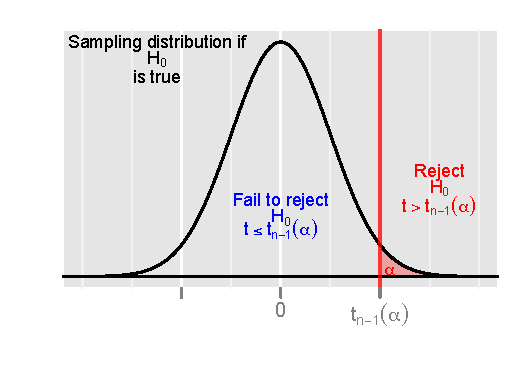
\includegraphics[width=0.5\textwidth]{diagram.pdf}}
%\caption{Decision regions  for classical inference for $H_0: \mu=\mu_0$ vs $H_a:\mu>\mu_0$.}
%\label{classical}
%\end{figure}
%
%\begin{figure}[hbtp]
%%\begin{figurehere}
%   \centering
%       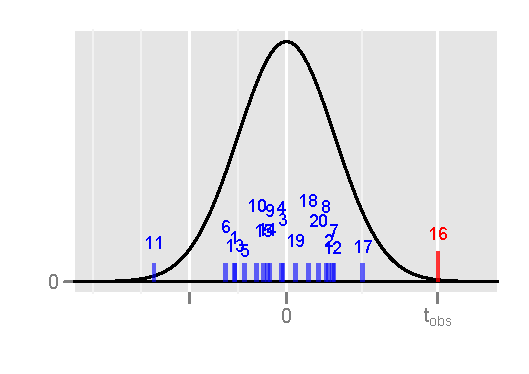
\includegraphics[width=0.5\textwidth]{visual-inference-plot-1.pdf}
%      \caption{Sampling distribution of the test statistic with the true value and the values for the null plots corresponding to the lineup in Figure \ref{lineup}.}
%      \label{visual-plot}
%%	\vspace{-.1in}
%\end{figure}

\begin{figure}[htbp]
\centering
\mbox{\subfigure[Classical Inference]{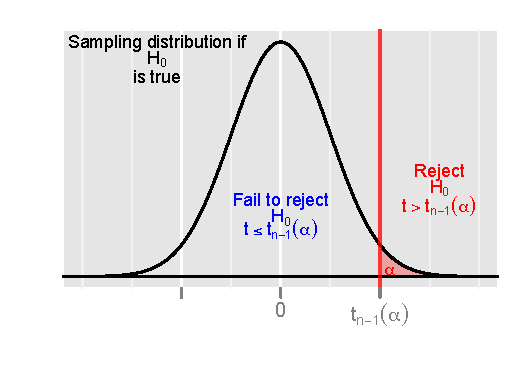
\includegraphics[width=3in]{diagram.pdf}}\quad
\subfigure[Visual Inference]{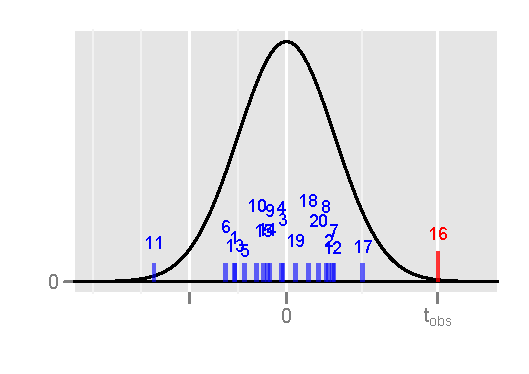
\includegraphics[width=3in]{visual-inference-plot-1.pdf} }}
\caption{Comparing the classical inference method and the visual inference method.  (a) gives decision regions  for classical inference for $H_0: \mu=\mu_0$ vs $H_a:\mu>\mu_0$ and (b) gives sampling distribution of the test statistic with the true value and the values for the null plots.  } 
\label{compare}
\end{figure}


***  Point 1: Finite comparison vs infinite comparison, measuring how different data plot is from null plots

In traditional hypothesis testing, the sampling distribution of the test statistics is continuous, which allows evaluation of probability on an infinite spectrum. With the lineup, although conceptually we may have an infinite collection of plots from the null distribution, in practice, we sample a finite number of null datasets to generate the lineup. A human judge has a physical limit on the number of null plots they can peruse. This poses one of the issues with using the lineup protocol.  Figure \ref{compare} is an attempt to compare the classical inference method and visual inference method. In classical inference setting, the black curve  gives the sampling distribution for the $t$-distribution under the null hypothesis with the regions for decision. In visual inference setting, let us consider that the black curve gives the sampling distribution although the sampling distribution is essentially a distribution of null plots. Although the test statistic is not numeric, the true data plot which is the test statistic is represented using red bar and the null plots that are drawn from the null distribution are the blue bars. % for the plots in the lineup shown in Figure \ref{lineup}. 
Effectively,  in visual inference the red line is compared only to these finite number of blue lines visually to make a decision, unlike classical inference where we look at the rejection region (Figure \ref{compare}) to make decisions. As Tukey suggested, `there is such a thing as a bad random sample' \citep{fernholz03}:

\begin{quotation}
There [in Tukey's Data Analysis class] I discovered that [...]  a random sample is indeed a ``batch of values'' which ``fail to be utopian'' most of the time.
\end{quotation}


***Point 2: Use metrics to ensure that a range of comparisons is made available to observers


To avoid basing conclusions on artifacts introduced by a `bad' sample, we need to be aware of properties of this set of null plots. In this paper, we develop techniques that help to determine the quality of the lineup. A variety of distance metrics measuring the ``closeness'' of the true data plot and the null plots, and the null plots with themselves are examined. These are compared to human subject picks in several Amazon Turk studies.  Describing plots numerically, is something  of an oxymoron, it cannot be done. Nonetheless, the distance measures provide indications of the quality of a lineup. The purpose of this paper is to help determine if a lineup might provide inadequate coverage of the full null distribution, and these measures might help to gain more insight on how the human eyes work in reading statistical graphics. The article is organized as follows. Section \ref{sec:null} discusses the null generating mechanisms. Section \ref{sec:meas} defines the distance measures and discusses the choice of the measures. The distribution of the distance measures are studied in Section \ref{sec:distri}. Section \ref{sec:plot_type} describes the effect of the plot type and the question of interest on the distance measure while Section \ref{sec:eval} talks about the distance evaluations. In Section \ref{sec:nbin}, the methods to select the number of bins for the binned distance is described. Section \ref{sec:results} presents a comparison of the distance measures to the performance of human subjects in several experiments conducted by Amazon's Mechanical Turk.

***  Point 3: Metrics might replace human observers, eventually, but as of now, human eye can still beat numbers for finding unexpected patterns. The lineup protocol gives us a chance to evaluate metrics to finding unexpected structures - check out the scagnostics literature

*** Point 4: Metrics can help us understand what it is that people pick up on to trigger a detection of the data. Currently lineups rely on people verbally reporting why they picked a plot. 

%Any statistical analysis must include some sreftatistical graphics. For exploratory data analysis, statistical graphics play an invaluable role in model checking and diagnostics. Even though we have established mathematical procedures to obtain various statistics, we need to support the results by also producing the relevant plots. 

%In recent times there have been major advances in statistical graphics. Modern computing systems like R and SAS produce high quality statistical graphics. Buja et al. 2009, following from Gelman 2004, proposed two protocols that allow the testing of discoveries made from statistical graphics.

%In this paper we are interested in the quality of a lineup plot. In visual inference, the actual plot is the test statistic and the lineup plot is the null distribution. Unlike classical inference, the null distribution is represented by the 19 null plots that we obtain randomly from the actual plot assuming that the null hypothesis is true. So the decision of rejection or failure of rejection of the null hypothesis is heavily dependent on these 19 null plots. This induces us to take a closer look at the null plots. For this purpose, we calculate different distance matrices between the null plots and the actual plot to get a measure on how close is each null plot to the actual plot. We also calculate the distance matrices between the null plots to see how close are the null plots to each often. Finally a percentile value is calculated to find how often such a distance appears in a lineup and a z-score of the different distances is calculated to get a measure on the closeness between the null plot and the actual plot and also compare between two different lineups.  

%In this paper we presents results of a human-subject study assessing the performance of the different distance matrices. Section \ref{sec:visual_test} describes the basic idea of the visual inference and also gives the definition of the different distance measures. Section \ref{sec:asso} and Section \ref{user.distance} applies these ideas and uses the definitions to calculate the different distance measures. In Section \ref{results} and Section \ref{sec:conclusions} we outline the setup and present results.

%\section{Visual Statistical Inference and Definitions} \label{sec:visual_test} 

%This section outlines the concepts of visual inference in comparison to the procedures of classical statistical inference and also gives the definition of the different distance measures. 

%Let $\theta$ be a population parameter of interest, with $\theta \in \Theta$, the parameter space. 
%Any null hypothesis $H_0$ then partitions the parameter space into $\Theta_0$ and $\Theta_0^c$, with $H_0: \theta \in \Theta_0$ versus $H_1: \theta \in \Theta_0^c$. 
% In hypothesis testing terminology, the parameter space $\Theta$ of a population parameter $\theta$, can be partitioned into $\Theta_0$ and $\Theta_0^c$. We test $H_0: \theta \in \Theta_0$ versus $H_1: \theta \in \Theta_0^c$.

%\subsection{Visual Statistic} 

%Unlike classical hypothesis testing, the statistic in visual inference is not a single value, but a plot that is appropriately chosen to describe the parameter of interest, $\theta$. When the alternative hypothesis is true, it is expected that the plot of the true data, the test statistic, will have visible feature(s) consistent with $\theta \in \Theta_0^c$, and that visual artifacts will not distinguish the test statistic as different when $H_1$ is not true.

%\begin{dfn}\label{dfn:lplot}
%A lineup plot is a layout of $m$ visual statistics, consisting of 
%\begin{itemize}\itemsep-3pt
%\item $m-1$ plots simulated from the model specified by $H_0$  (null plots) and 
%\item the test statistic produced by plotting the true data, possibly arising from $H_1$.
%\end{itemize}
%\end{dfn}

%If $H_1$ is true, the test statistic is expected to be the plot that is most different from the other plots in the lineup plot. A careful visual inspection should reveal the differences in the feature shown by the test statistic under null and alternative hypothesis. {\em If the test statistic cannot be identified} in the lineup, the conclusion is to {\em not reject the null hypothesis.} The $(m-1)$ null plots can be considered to be samples drawn from the sampling distribution of the test statistic assuming that the null hypothesis is true. \\

%Since the lineup plot consists of $m$ plots, the probability of choosing any one of them is $1/m$. Thus we have a type-I error probability of $1/m$.

%\red{the next three paragraphs might be important, but you loose focus - you want to come as fast as possible to the problematic of the paper, e.g.:}
%The lineup plot can be evaluated by one or more individuals. When a single individual identifies the true graph in the lineup plot we report a $p$-value of at most $1/m$, otherwise the $p$-value is at least $1-\frac 1m$. 
%
%If $N$ individuals evaluate a lineup plot independently, we count the number of successful evaluations as $U \sim \text{Binom} (N,\frac{1}{m})$ and report a  $p$-value of at most $Pr(U \ge u)= \sum_{k \ge u}^N {{N \choose k} (\frac{1}{m})^k(1-\frac 1m)^{(N-k)}}$ where $u$ is the true number of successful evaluations. %Notice that when $N=1$, this $p$-value is $\frac1m$.  \\ 
%
%
%For two different visual test statistics of the same true data, the one  is better, in which a specific pattern is more easily distinguishable visually. \\ \\

%\red{Before distance measures are introduced, introduce the problem of why we look at these distances in the context of permutation tests. }
%The difference between a regular permutation test and a graphical test under the line-up protocol, is that we are comparing the true value of the test statistics (i.e. the plot of the true data) to a finite sample of the sample distribution.

%{\color{red} Things to add:
%\begin{enumerate}
%\item Null-generating mechanisms 
%\item Dependence on Question of Interest - in general should not be a problem because the question is ``which is different? ". But for data from Turk study, questions were quite focussed.
%\item Interplay between type of plot and distance metric - calculation on data vs graphical elements. For example, scatterplot vs reg line distance
%\item Distance metric distribution calculation eg permutation
%\item Selection of the number of bins
%\end{enumerate}}

\section{Null Generating Mechanism} \label{sec:null}

The lineup protocol embeds the true data plot among a set of null plots. The method of obtaining these null plots is known as the null generating mechanism. These null plots are obtained from the null distribution in a method consistent with the null hypothesis. The null hypothesis directly affects the method of generating null plots. This can be done in a few different ways:
\begin{itemize}
\item Permutation: This is the most common approach. Consider two variables $X$ and $Y$. In this method,  either $X$ or $Y$ is permuted keeping the other variable fixed. Any association between $X$ and $Y$ is broken in the process. The marginal distribution of $X$ and $Y$ stay the same while the joint distribution is altered. The method works in situations where one or both the variables are continuous or categorical. Let us consider a case where we have one categorical variable, say, Group and a continuous variable. Let us assume that the variable Group has two levels (say, A and B) and we want to test whether there is any significant difference between the two groups, i.e. $H_o: \mu_A = \mu_B$. To generate the null in this case,  the variable Group can be permuted keeping the continuous variable fixed. 
\item Simulation under the null model: Simulation from the null model is another approach. Assuming that the null hypothesis is true, the model is fitted to the true data. The parameter estimates are obtained from the fitted model and then the data is generated using the parameter estimates. Let us consider that we are interested in testing whether there is any significant linear relationship between two continuous variables $X$ and $Y$. Hence we test for $H_o : \beta_1 = 0$ versus $H_a: \beta_1 \ne 0$. Under the null hypothesis, we fit the following model to the data:
$$Y = \beta_0 + \varepsilon$$
where $\varepsilon \sim \hbox{Normal}(0, \sigma^2)$. The parameter estimates of $\beta_0$ and $\sigma^2$ are obtained and the null data is generated from $\hbox{Normal}(\widehat{\beta_0}, \widehat{\sigma}^2)$. 
\item Simulation from a specific distribution: The null data can also be simulated from a specific distribution depending on the null hypothesis. This method is mainly is used in situations where the null hypothesis is that the data comes from a specific distribution. The parameters for the null distribution is obtained from the parameter estimates from the data. For example, suppose we want to test whether data comes from a Normal distribution. Hence $H_o:$ data $\sim$ Normal vs. $H_A:$ data $\nsim$ Normal. Hence the null data are generated from the Normal distribution with mean and standard deviation equal to the estimated mean and standard deviation from the data. 
\end{itemize} 

There may be other null generating mechanism depending on the hypothesis. 

\section{Distance measures} \label{sec:meas}

%\blue{The difference between a regular permutation test and a graphical test under the line-up protocol, is that we are comparing the true value of the test statistics (i.e. the plot of the original data) to a finite sample of the sample distribution. As Tukey suggested, `there is such a thing as a bad random sample' \citet{fernholz03}:
%\begin{quotation}
%There [in Tukey's Data Analysis class] I discovered that [...]  a random sample is indeed a ``batch of values" which ``fail to be utopian" most of the time.
%\end{quotation}
%
%To avoid basing our conclusion on artifacts introduced by a `bad' sample, we need to be aware of properties of this set of null plots. In this paper, we are proposing a set of  distance measures that help us in the evaluation of the goodness of a random sample. It also turns out, that these measures give us also some insight in the perceived difficulty of picking the original plot of the data from a particular line-up. 
%
%\subsection*{Distance Measures}
%}

%\red{The distance measures need some more setting up beforehand. I would actually include a small example of a set of scatterplots that highlights the problematic.}
%
%\red{Another thing that we should discuss on Friday is whether it might be better to call the measures we use norms rather than distances - a distance usually assumes the comparison of two objects, and we implicitly compare against null or identity, which is what a norm does..}

There are different types of distance measures suitable in measuring the distance between the null data and the true data. In this paper, six different types of distance measures were used so that they can identify the different characteristics present in a plot. \\

For all of the distance measures below, let $X$ denote the true dataset with one or two variables. Let $Y$ denote the null dataset obtained from $X$ using any of the above mentioned null generating mechanism.

%\blue{For all of the distance measures below, let $P$ be a permutation mapping  the set $\{1, 2, ..., n\}$ onto itself. Let further $[P]$ denote the $n \times n$ matrix associated to permutation $P$.
%}
\begin{itemize}

%\item Hamming Distance: The hamming distance $H$ of $P$ is defined as 
%\[
%H(P) := \sum_{i=1}^n I_{P(i) \neq i},  \text{ where } I_{x} = \left \{ 
%\begin{array}{ll}
%1 & \text{if } x \text{ is true},\\
%0 & \text{otherwise},
%\end{array} \right.
%\]
%i.e. $H(P)$ is a count of the number of fix elements of the function.


%\blue{
%The hamming distance $H$ of $P$ is defined as 
%\[
%H(P) := \sum_{i=1}^n I_{P(i) \neq i},  \text{ where } I_{x} = \left \{ 
%\begin{array}{ll}
%1 & \text{if } x \text{ is true},\\
%0 & \text{otherwise},
%\end{array} \right.
%\]
%i.e. $H(P)$ is a count of the number of fix elements of the function.
% }

%Hamming distance between two equal length strings is the number of positions at which the corresponding symbols are different. 

%This distance matrix measures the distance between the permutation matrix and the identity and does not depend on the actual values of the variables $X$ and $Y$. 


%\blue{let $X$ be a continuous variable. The Euclidean Distance under permutation is then defined as 
%%\red{we need a good short-cut for this distance}
%\[
%d^2_P(X) := || X - [P]X||^2 = \sum_{i=1}^n (X_i - X_{P(i)})^2.
%\]
%}

%\item Euclidean Distance: 
%Let $X$ be a continuous variable. The Euclidean Distance under permutation is then defined as 
%%\red{we need a good short-cut for this distance}
%\[
%d^2_P(X) := || X - [P]X||^2 = \sum_{i=1}^n (X_i - X_{P(i)})^2.
%\]



%Euclidean Distance between two equal length strings measure the distance between the permuted values of one variable and the original continuous variable while the other variable, either continuous or categorical, remains unaltered. This distance matrix takes into  account the actual values of the variable that is permuted and does not depend on the values of the other variable. 

\item Binned Distance:
%\red{write out mathematically, include all definitions - i.e. C(X,Y) needs to be defined - have a look at the grammar of graphics}
Let $X_1$ and $X_2$ be two continuous variables. Let $X_1$ be divided into $p$ bins and $X_2$ divided into $q$ bins. $(i,j)$-th cell represents the $j$-th bin of $X_2$ corresponding to the $i$-th bin of $X_1$. Let $C(X_1,X_2)$ be defined as a $p \times q$ matrix. Each $(i,j)$-th element of the matrix represents the number of points falling in the $(i,j)$-th cell, where $i = 1, \dots, p$ , $j = 1, \dots, q$.
The Binned distance is then defined as
\begin{eqnarray*}
d_{\hbox{bin}}^2 (X, Y) &:=& ||C_X(X_1, X_2) - C_Y(X_1,X_2)||^2 \\ &=& \sum_{i=1}^p \sum_{j=1}^q (C_X(X_{1i},X_{2j}) - C_Y(X_{1i},X_{2j}))^2.
\end{eqnarray*}
Binned distance is highly susceptible to small differences in values and depends on the number of bins as well as exact cut-offs. This is particularly problematic for small number of points. As a remedy to that, we are considering Weighted bin distance next, which is based on the density rather than point frequency. For large number of points the weighted binning is computationally too intensive, in which case we will make use of the unweighted binned distance.
%\red{careful: $C(X,[P]Y)$ is not the same as $C_{i,P(j)}$. $C_{i,j}$ is the count for points falling into cell $i,j$ - it's not enough to permute the grid counts, we need to get the grid counts of the permuted variable. Introduce $C$ as a function of $X$ and $Y$ ....}

% To calculate this distance, we form a $p \times q$ grid between the two continuous variable and count the number of points falling to each grid. Then we permute one continuous variable keeping the other variable unchanged and repeat the above procedure. The euclidean distance between the counts for the original and permuted data gives an measure of the binned distance. Binned distance takes into account both the variables but only one of the variables is permuted. Binned distance considers only the count for each respective bin and puts no weight on the counts of the neighboring bin.

\item Weighted Bin Distance: Using the same setup of the binned distance, the weighted bin distance is defined as 
\begin{eqnarray*}
d_{\hbox{wbin}}^2(X, Y) &:=&||W_X(X_1,X_2) - W_Y(X_1,X_2))||^2 \\ &=& \sum_{i=1}^n (W_X(X_{1i},X_{2i}) - W_Y(X_{1i},X_{2i}))^2 , 
\end{eqnarray*}
where $W(X_{1i},X_{2i})$ denotes the joint (empirical) density of $X_1$, $X_2$ at location $(X_{1i}, X_{2i})$. See Figure \ref{fig:test_category} for a comparison of weighted and unweighted binned distance at the example of 20  points.
%The weighted bin distance is an improvement to the bin distance where a weight is provided to the counts of the neighboring bins. The weight is done by doing a kernel density estimation of the different bins.

%\green{I wrote something down here but I am not sure if this works.}

\begin{figure}[hbt]
%\begin{figurehere}
   \centering
       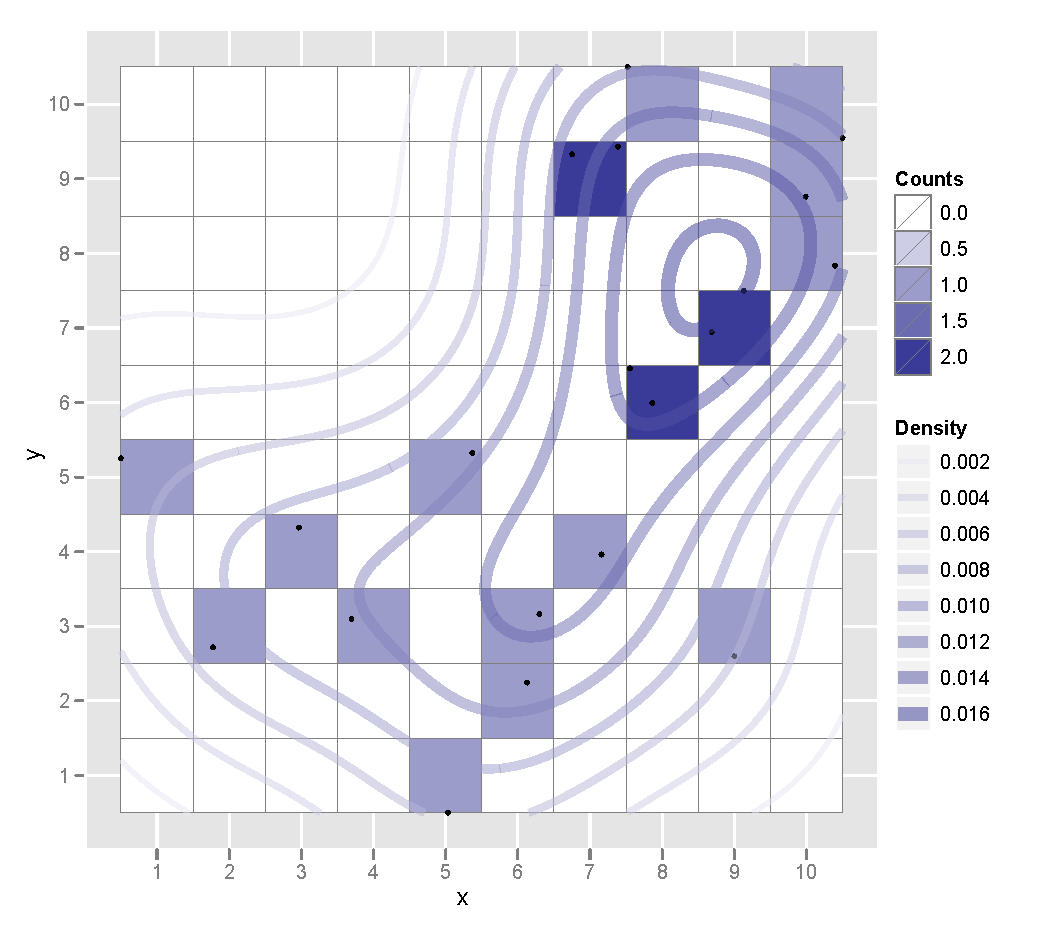
\includegraphics[width=3.3in]{wbdist.pdf}
	\vspace{-.2in}
       \caption{Scatterplot of 20 points in $X_1$ and $X_2$ with a weak positive association. The colored tiles show binned frequencies, the contour lines show two-dimensional density.}
       \label{fig:test_category}
\end{figure}


\item Hausdorff distance: Let $x \in X$ and $y \in Y$ be two sets of points. The Hausdorff distance between $X$ and $Y$ is defined as
 \[
d_{\hbox{hausdorff}}(X, Y)  = max (h(X, Y), h(Y, X))
\]
where 
\begin{eqnarray*}
h(X, Y) &:=& \max_{x \in X} \min_{y \in Y} ||x - y|| \\ & = & \max_{x \in X} \min_{y \in Y} \sqrt{\sum_{i=1}^n (x_i - y_i)^2}
\end{eqnarray*}

This measure is computationally intensive.

\end{itemize}

%The remaining distance measures are different from the ones above, in that they are used to directly draw inference on a linear association between variables $X$ and $Y$, whereas the other ones were not specifically tailored to this purpose.

%\blue{The remaining distance measures are different from the ones above, in that they are used to directly draw inference on a linear association between variables $X$ and $Y$, whereas the other ones were not specifically tailored to this purpose.}
The remaining distance measures are different from the ones above, in that they are used for specific plot types and cannot be used for any type of data. The following distance measures uses the graphical element to calculate the distances.

\begin{itemize}
\item Distance for univariate data: Let $X$ be a continuous variable. Then the distance metric is given by
\[
d^2_{\hbox{uni}}(X, Y) := ||m(X) - m(Y)||^2 = \sum_{i=1}^4 ((m(X))_i - (m(Y))_i)^2
\]
where $m(.)$ is a vector of the mean, the standard deviation, the skewness and the kurtosis of the variable. This distance metric works for univariate distributions using only the graphical elements in the plot.


\item Distance based on boxplots : Let $X_1$ be a categorical variable representing the groups in the data and $X_2$ be a continuous variable. Then the distance metric is given by
 \[
d^2_{\hbox{box}}(X, Y) := || d_q(X) - d_q(Y)||^2 = \sum_{i=1}^3 ((d_q(X))_i - (d_q(Y))_i)^2
\]

where $d_q(.)$ is a vector giving the absolute difference of the first quartile, median and the third quartile of $X_2$ between the two groups in $X_1$. This distance measure works specifically for the boxplots using only the graphical elements. This is based on the assumption that after the boxplots have already been constructed, the subjects only look at the difference in the boxes to make the distinction. 


\item Distance based on the regression line: Let $X_1$ and $X_2$ be two continuous variables. $X_1$ and $X_2$ are plotted in a scatterplot and assume that the scatterplot is binned vertically into $b$ bins. In each vertical bin, a linear regression model is fitted and the regression coefficients i.e. the estimated intercept and the estimated slope are noted. The distance metric based on the regression coefficients is given by
 \[
d^2_{\hbox{reg}}(X, Y) := \hbox{tr} (B(X) - B(Y))' (B(X) - B(Y)) = \sum_{i=1}^b ((b_0(X))_i - (b_0(Y))_i)^2 + \sum_{i=1}^b ((b_1(X))_i - (b_1(Y))_i)^2
\]

where $b_0$ and $b_1$ denote the vector of the intercept and slope respectively while $b$ is the number of bins. $B(.)$ is a $b \times 2$ matrix of the regression coefficients where each row represent the  intercept and the slope obtained from each bin. The number of bins have a significant effect on the distance measure. It can be seen that it works best for smaller number of bins like 1 or 2. With larger number of bins (i.e. smaller bin sizes), the regression coefficients are affected by the skewness of the data.

\end{itemize}

The last two distance measures are also dependent on the question of interest and hence can be changed accordingly. But in general this should not be a problem because the question is ``Which plot among these is different ?". 
%\item $t$ statistic: In this paper we used the test statistic of a t-test based on the correlation coefficient $r$ where $$t =\frac{r \sqrt{n - 2}}{\sqrt{1 - r^2}}$$ where $n$ is the number of observations in $X$ or $Y$. This is the only measure that makes a distributional assumption that the ($X$,$Y$) follows approximately a bivariate Normal distribution. Hence the $t$-statistic follows a t distribution with ($n$ - 2) degrees of freedom.
%%\red{use either upper case or lower case $T$, not both. }
%%The first one was used when one variable is continuous and the other is categorical while the other is used when both the variables are continuous.  
%
%%\item Wilcoxon Rank Sum Test statistic: This is a nonparametric test statistic for assessing whether one of the two samples of independent observations tend to have larger values than the other. This is also used when one variable is continuous and the other is categorical.  
%
%\item Spearman's rank correlation $\rho$ : $\rho$ is a nonparametric alternative to the correlation coefficient with Kendall's $\tau$. $X$ and $Y$ are converted into the ranks $x$ and $y$. Assuming there are no ties in the data, the differences $d_i=x_i - y_i$ between the ranks of each observation between the two variables are calculated and $\rho$ is given as $$\rho = 1 - \frac{6\sum_{i=1}^n d_i^2}{n(n^2 - 1)}$$ The Spearman's rank correlation is a better measure of correlation than the Pearson's rank correlation if the data contains some outliers. Kendall's $\tau$ is computationally intensive
%% - the naive implementation is $O(n^2)$, but it can be reduced to $O(n \log n)$, which is equivalent to sorting.}
%%takes huge time \red{could you be more specific - is it $O(n^2)$? - I think it can be brought down to $O(n \log n)$} \green{I think I used 2 for loops. So it should be $O(n^2)$. But I am not sure if it can be brought down to $O(n \log n)$}to calculate for an averaged size sample. 
%So in this paper we considered $\rho$ as the only nonparametric measure.
%%\red{which one of the statistics do you refer to?} 
%%\red{give a mathematical definition of $\rho$}
%$\rho$ uses both the variables. 
%
%
%\item Euclidean Distance of permutations: The Euclidean distance of permutations $P$ is 
%\[
%d^2_P(X) = \sum_{i=1}^n ( i - P(i))^2.
%\]
%where $i = \{1, 2, ..., n\}$
%
%
%\item Canberra Distance: Using exactly the same setup as the binned distance , the canberra distance under permutation is defined as
%%\begin{eqnarray*}
%\[
%c^2_P(X)  = \left \{ 
%\begin{array}{ll}
%\sum_{i=1}^p \sum_{j=1}^q \frac{ |C_{X_i,Y_j} - C_{X_i,P(Y)_j}|}{ C_{X_i,Y_j} + C_{X_i,P(Y)_j}} & \text{if } C_{X_i,Y_j} + C_{X_i,P(Y)_j} > 0,\\
%0 & \text{otherwise},
%\end{array} \right.
%\]
%Like the binned distance, the canberra distance is also effected by the number of bins used. Here again we use the usual convention as the binned distance. Canberra distance is an improvement to the binned distance as it puts less weight on the bins which has a large number of points than the bins with fewer points. Visually it is difficult to differentiate between a single point and a number of points having the exact coordinates. Canberra distance has the same drawbacks as the binned distance. So we defined the weighted canberra distance which is a similar measure as the weighted bin distance.
%
%\item Weighted Canberra Distance:  Using the same setup of the weighted bin distance, the weighted canberra distance under permutation is defined as 
%%\begin{eqnarray*}
%\[
%wc_P^2(X) = \left \{ 
%\begin{array}{ll}
%\sum_{i=1}^p \sum_{j=1}^q \frac{ |W_{X_i,Y_j} - W_{X_i,P(Y)_j}|}{ W_{X_i,Y_j} + W_{X_i,P(Y)_j}} & \text{if } W_{X_i,Y_j} + W_{X_i,P(Y)_j} > 0,\\
%0 & \text{otherwise},
%\end{array} \right.
%\] 
%%\end{eqnarray*}
%where like the weighted bin distance, $W_{X_i,Y_i}$ denotes the joint (empirical) density of $X$, $Y$ at location $(X_i, Y_i)$. 
%
%\item Correlation between $Y$ and $[P]Y$: Let $Y$ be a continuous variable.The correlation between the $Y$ and $[P]Y$ is defined as
%\[
%r_P(X) = \frac{ \sum_{i=1}^n (Y_i - \bar{Y_i})(Y_{P(i)} - \bar{Y}_{P(i)})}{\sqrt{\sum_{i=1}^n (Y_i - \bar{Y_i})^2}\sqrt{\sum_{i=1}^n (Y_{P(i)}- \bar{Y}_{P(i)})^2}}.
%\]



\section{Distance metric distribution} \label{sec:distri}

The empirical distribution of the distance measures may be obtained by calculating the distances between the null plots among themselves. One null data is generated from the true data set using the null generating mechanism. Assuming this null data to be the ``true" data set, a number of null data sets are obtained from this null data and the distances between these datasets are calculated. One single distance value is obtained by averaging all these distances. This process is repeated a large number of times, say, $N$ where $N$ is a large number of the order $10^3$ or $10^4$. Finally $N$ mean distances or average distances are obtained which gives the empirical distribution of the distance. 

The empirical distribution of the distance works as the $t$-distribution in the classical setting. In the classical setting, the test statistics follows a $t$-distribution under the null hypothesis. The observed test statistic is then compared to this distribution, as shown in Figure \ref{compare}. In visual inference, the mean distances of the null plots gives the empirical distribution. The mean distance of the true plot from the null plots in the lineup acts as the observed test statistic. Unlike the $t$-distribution, the empirical distribution is generally skewed.

The mean distance between the true plot and the null plots in a lineup of size $m = 20$ is calculated by averaging over the distances between the true plot and each of the  $(m - 1)$ null plots. The mean distances for the $(m - 1)$ null plots in the lineup are calculated by taking the mean of the distances of the particular null plot and the other $(m - 2)$ null plots. The mean distances for the true dataset and the null datasets are plotted on the empirical distribution. If the mean distance of the true plot is larger than any of the null plots, the lineup would be regarded as``easy". Otherwise, it is a ``difficult" lineup. 

The empirical distribution of the distance based on regression is shown in Figure \ref{dist}. To generate this distribution, $N = 1000$ and $m = 20$ was used. Figure \ref{dist_1} shows the lineup plot for $m = 20$ for testing whether there exists a significant linear relationship between $X_1$ and $X_2$. The 19 null plots are generated by fitting the null model and generating from the null model. Figure \ref{dist_2} shows the empirical distribution of the distance with the mean distances for the true plot (in orange) and the null plots (in black) for the particular. The true plot is easy to be identified in the lineup (Figure \ref{dist_1}). It can also be seen in Figure \ref{dist_2} as the orange line is extreme compared to the black lines. 

\begin{figure*}[hbtp]
\centering
\subfigure[]{
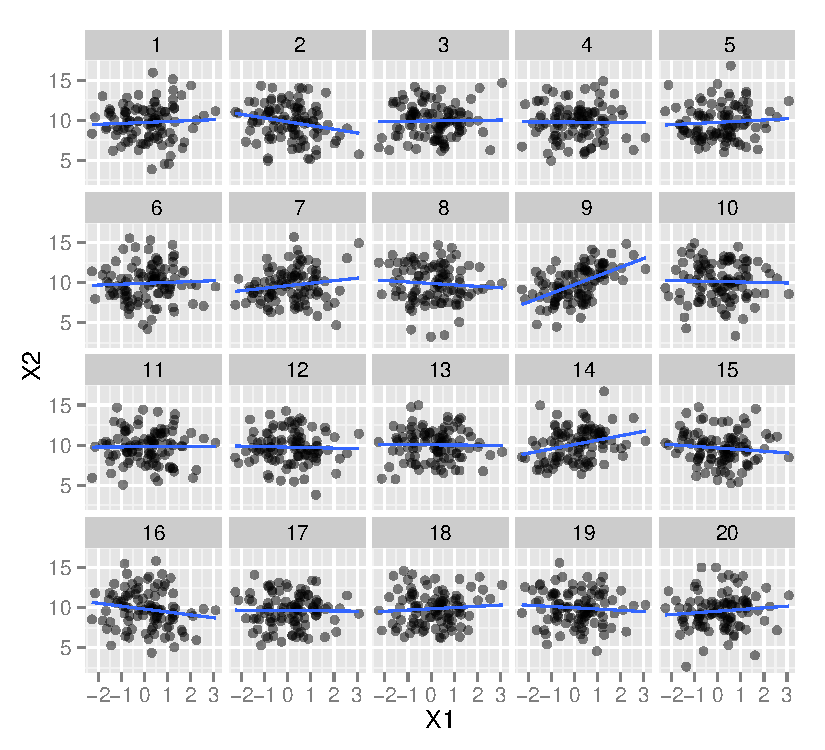
\includegraphics[scale=0.55]{dist-example.pdf}
\label{dist_1}
}
\subfigure[]{
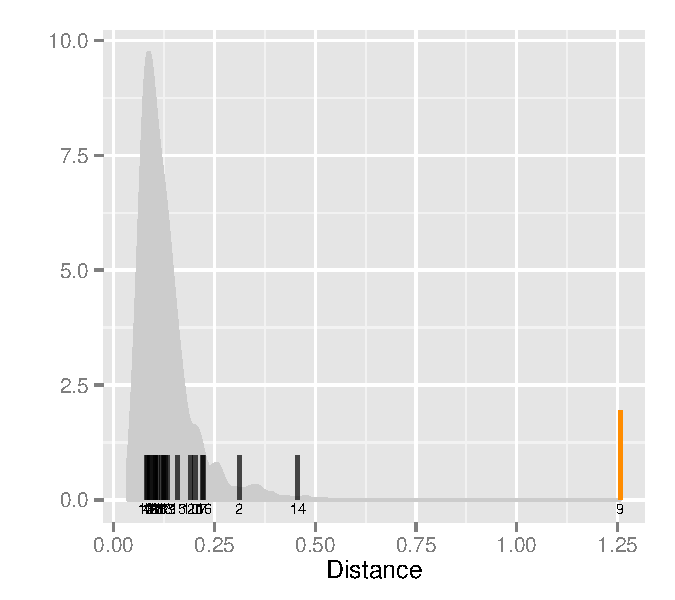
\includegraphics[scale=0.7]{dist-metric.pdf}
\label{dist_2}
}
\label{dist}
	\vspace{-.1in}
\caption[Optional caption for list of figures]{(a) Lineup Plot ($m$ = 20) for testing whether there exists a significant linear relationship between $X_1$ and $X_2$. The 19 null plots are obtained by simulating from the null model.  (b) The chart on the right shows the empirical distribution of the distance based on regression parameters. The distance of the true plot is shown in orange while the distance for the null plots are shown in black. }
%{Caption of subfigures \subref{fig:subfig1}, \subref{fig:subfig2} and \subref{fig:subfig3}}
\end{figure*}

\begin{figure*}[hbtp]
\centering
\subfigure[]{
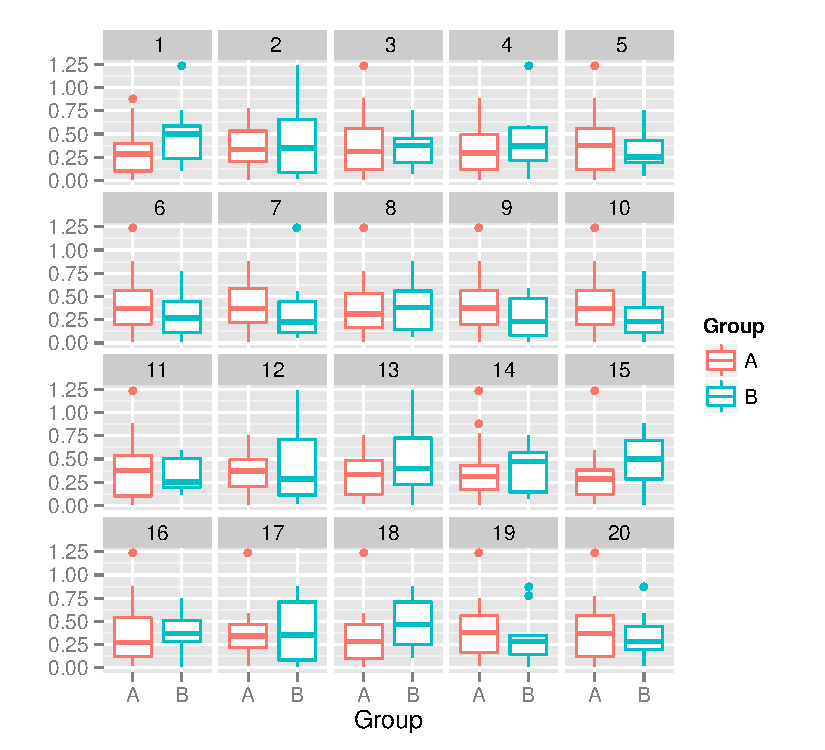
\includegraphics[scale=0.55]{dist-example-2.pdf}
\label{dist2_1}
}
\subfigure[]{
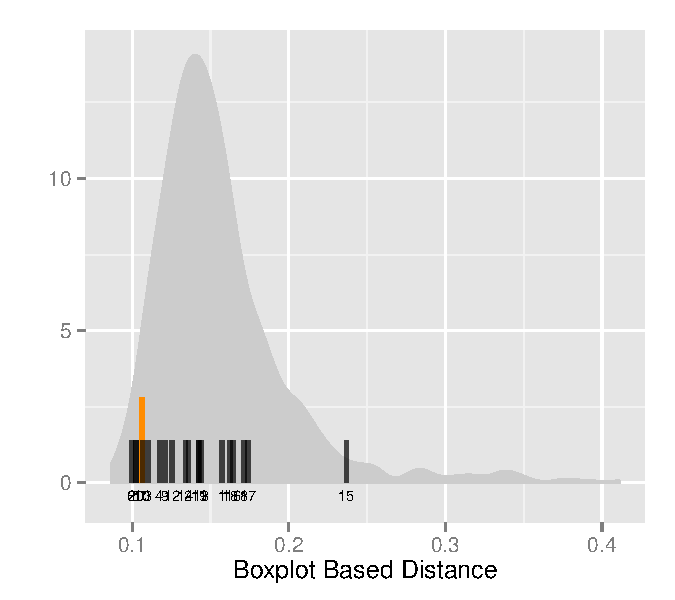
\includegraphics[scale=0.7]{dist-metric-2.pdf}
\label{dist2_2}
}
\label{dist2}
	\vspace{-.1in}
\caption[Optional caption for list of figures]{(a) Lineup Plot ($m$ = 20) for testing whether there exists a significant difference between the two groups A and B. The 19 null plots are obtained by permuting the group variable while keeping the continuous variable fixed.  (b) The chart on the right shows the empirical distribution of the distance based on boxplots. The distance of the true plot is shown in orange while the distance for the null plots are shown in black. }
%{Caption of subfigures \subref{fig:subfig1}, \subref{fig:subfig2} and \subref{fig:subfig3}}
\end{figure*}

Figure \ref{dist2_1} shows the lineup plot for $m = 20$ for testing whether there exists a significant difference between the two groups A and B. The 19 null plots are generated by permuting the group variable keeping the other variable fixed. Figure \ref{dist2_2} shows the empirical distribution of the distance based on the boxplots with the mean distance for the true plot (in orange) and the null plots (in black). The true plot is hard to be identified from the lineup which is also evident in the distribution since many black lines are to the right of the orange line.

\section{Effect of Plot type and Question of interest } \label{sec:plot_type}

Previous studies have suggested that the type of plot used in the lineup have an effect on the response of the subjects \citep{zhao:2012}. For example the subjects find it easier to identify the true plot for a large sample data when a box plot is used in the lineup instead of a dot plot. Similarly the distance metric should also be altered according to the plot type. The distance metric should account for the additional information provided by the graphical elements in the lineup. The graphical elements, like the presence of a box or a regression line overlaid on a scatterplot may influence the response of the subject. Figure \ref{plottype} illustrates this idea. 

\begin{figure*}[hbtp]
\centering
\subfigure[]{
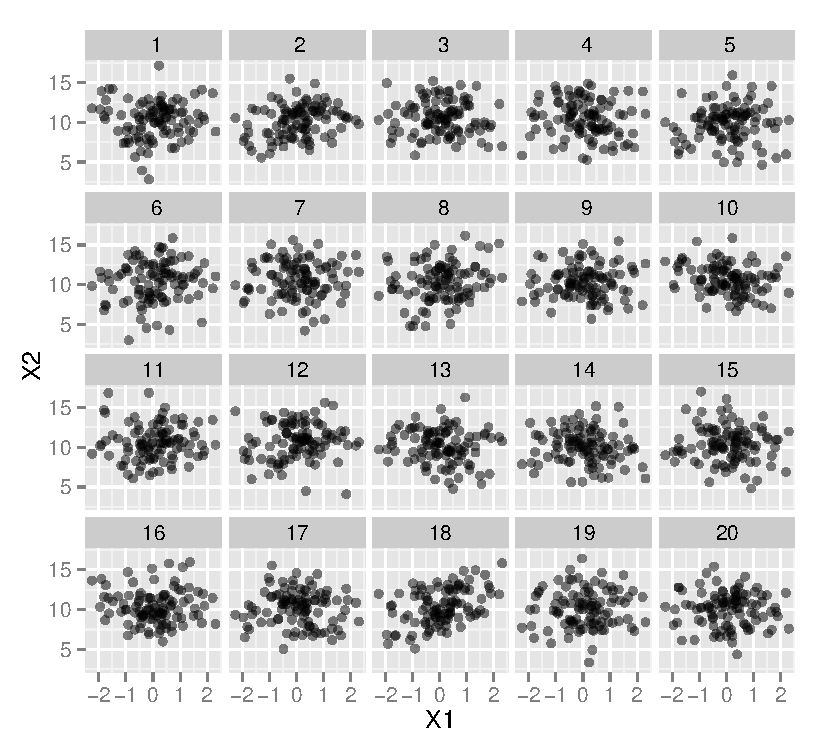
\includegraphics[scale=0.55]{plot-type-sca.pdf}
\label{type_1}
}
\subfigure[]{
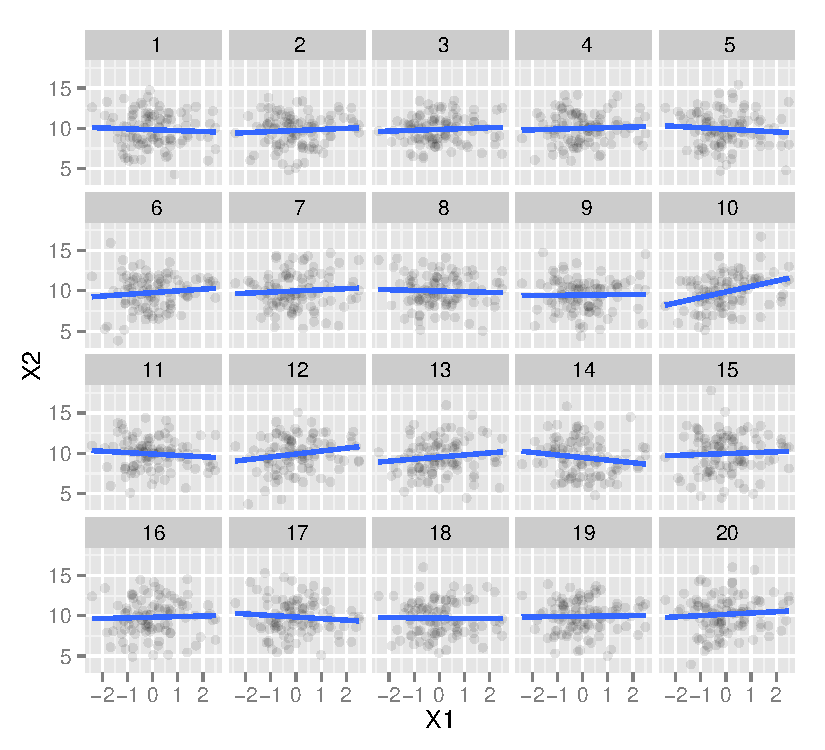
\includegraphics[scale=0.55]{plot-type-reg-line.pdf}
\label{type_2}
}
\label{plottype}
	\vspace{-.1in}
\caption[Optional caption for list of figures]{(a) Lineup Plot ($m$ = 20) for testing whether there exists a significant difference between the two groups. The 19 null plots are obtained by permuting the group variable while keeping the other variable fixed.  (b) The chart on the right shows the empirical distribution of the distance based on boxplots. The distance of the true plot is shown in orange while the distance for the null plots are shown in black. }
%{Caption of subfigures \subref{fig:subfig1}, \subref{fig:subfig2} and \subref{fig:subfig3}}
\end{figure*}

Figure \ref{type_1} shows a lineup of scatterplots with 100 points between two variables $X_1$ and $X_2$. Figure \ref{type_2}, on the other hand, gives a lineup of the same scatterplots with the regression line overlaid. Showing Figure \ref{type_1}, if the subjects are asked to identify the plot which has the steepest slope, then the subjects probably will face some difficulty in identifying the true plot. But in Figure \ref{type_2}, the regression line overlaid makes it easier for the subjects to identify the true plot. A different distance metric should be used in each case to correctly measure the quality of the lineup.

The question asked to the subjects plays an important role to identify the true plot in the lineup. A minor change in the question can change the response of the subject. In Figure \ref{dist2_1}, if the subjects are asked to identify the plot in which the green group has a larger vertical difference than the red group, the subjects should pick Plot 6. If the subjects are asked which plot has the largest vertical difference between the two groups, the subjects should pick Plot 15. A distance metric should also take into account the question of interest. But, in general, the question of interest is which plot among these is different.

\section{Metric Evaluation} \label{sec:eval}

For a lineup of size $m = 20$, the distance for the true plot is compared to the 19 null plots. This comparison can sometimes complicate things. A logical solution can be to look at one statistic for one lineup. Such a statistic can be defined as the difference between the mean distance of the true plot and maximum of the mean distances for the null plots. Hence we define, 
\begin{enumerate}
\item Difference: the difference between the mean distance for the true plot and the maximum of the mean distances for the null plots. Mathematically,
$$\delta_{\hbox{lineup}} = \bar{d}_{\hbox{true}} - \max_j \bar{d}_{\hbox{null}_j}$$
for $j = 1, \dots, (m  - 1).$
 A positive difference would indicate that the mean distance of the true plot is greater than the maximum of the mean distances of the null plots. Hence the true plot is extreme compared to all the null plots. Similarly a negative difference indicates that there is at least one null plot which is extreme compared to the true plot based on the distance.
 
The issue with this statistic is that $\delta_{\hbox{lineup}}$ indicates an ``easy" or ``difficult" lineup only on the basis of whether it is positive or negative, although it may be really close to 0. The statistic does not imply how many null plots are more extreme than the true plot. So we define,
\item Larger than the true plot: the number of null plots which have larger mean distances than the mean distance of the true plot is noted. Mathematically,
 $$\gamma_{\hbox{lineup}} = \sum_{j = 1}^{m - 1} a_j$$ where 
\begin{equation}
a_j =
\begin{cases}
1 & \text{if } \bar{d}_{\hbox{null}_j} > \bar{d}_{\hbox{true}} ,
\\
0 & \text{otherwise}
\end{cases}
\end{equation}
$\gamma_{\hbox{lineup}}$ takes all values between 0 and $(m - 1)$. A large value of this measure would indicate that there are a number of null plots more extreme than the true plot and hence it is hard to identify the true plot in the lineup.
\end{enumerate}


%\newpage

\section{Selection of the number of bins} \label{sec:nbin}

Binned distance works for any type of data and for any null generating mechanism. It does not take into account the graphical elements in the plot, and the raw data is used. Binned distance can be used in situations where no distance measure is known for the particular plot type and hence it can be regarded as universal. But the choice of number of bins or the bin size highly affects the distance. A wrong choice may produce erroneous or conflicting results. Hence the choice of the number of bins is important.

The choice of number of bins or bin sizes is investigated with different types of data. Different null generating mechanisms are also used for the same data type. Null datasets are obtained for a true data using a null generating mechanism and hence a lineup is constructed. Mean binned distance is calculated between the true data and the null datasets and also among the null datasets. The number of bins for the binned distance are varied from 2 to 10 on both $x$ and $y$ direction and $\delta_{\hbox{lineup}}$ is calculated for each combination. Table \ref{tbl:bin1} and Table \ref{tbl:bin2} shows the type of data, the observed plot, the null generating mechanism, a typical null plot, the difference $\delta_{\hbox{lineup}}$ and also the maximum value of $\delta_{\hbox{lineup}}$, the $x$-bin and $y$-bin for which the maximum was obtained. The minimum $\delta_{\hbox{lineup}}$ is also reported to get an idea of the range of values.

%\begin{figure*}[hbtp]
%\centering
%\subfigure[]{
%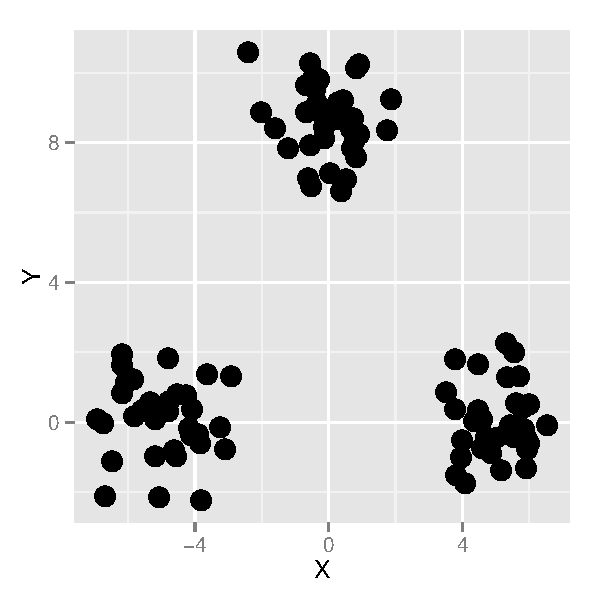
\includegraphics[scale=0.55]{data1.pdf}
%\label{nbin1_a}
%}
%\subfigure[]{
%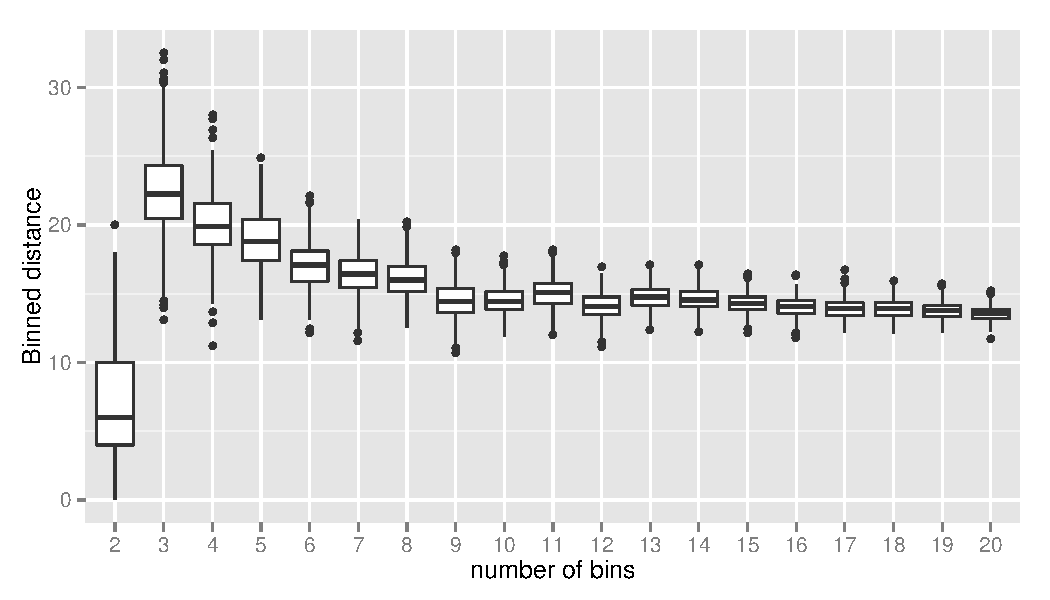
\includegraphics[scale=0.55]{data1-nbin.pdf}
%\label{nbin1_b}
%}
%\label{nbin1}
%	\vspace{-.1in}
%\caption[Optional caption for list of figures]{(a) Plot showing the observed data (b) Binned distance plotted against the number of bins. }
%%{Caption of subfigures \subref{fig:subfig1}, \subref{fig:subfig2} and \subref{fig:subfig3}}
%\end{figure*}
%
%\begin{figure*}[hbtp]
%\centering
%\subfigure[]{
%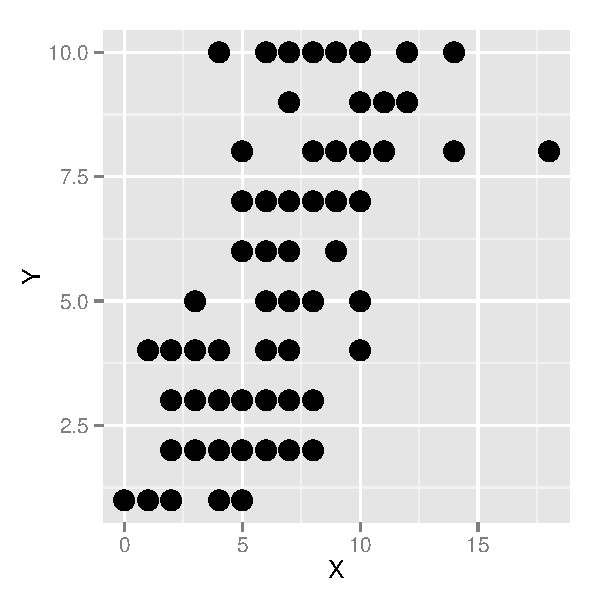
\includegraphics[scale=0.55]{data2.pdf}
%\label{nbin2_a}
%}
%\subfigure[]{
%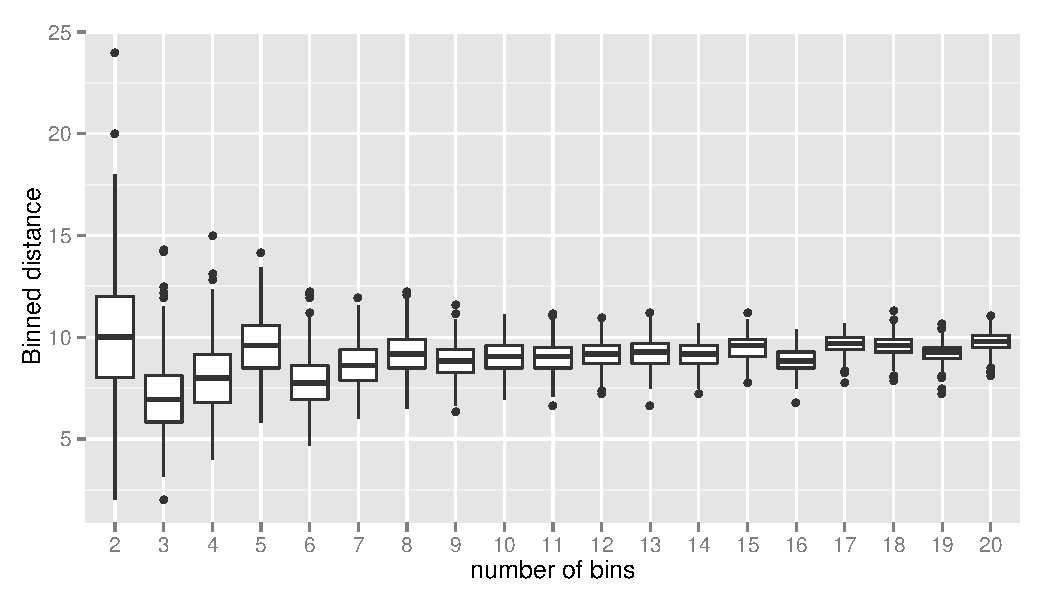
\includegraphics[scale=0.55]{data2-nbin.pdf}
%\label{nbin2_b}
%}
%\label{nbin2}
%	\vspace{-.1in}
%\caption[Optional caption for list of figures]{(a) Plot showing the observed data (b) Binned distance plotted against the number of bins. }
%%{Caption of subfigures \subref{fig:subfig1}, \subref{fig:subfig2} and \subref{fig:subfig3}}
%\end{figure*}
%
%\begin{figure*}[hbtp]
%\centering
%\subfigure[]{
%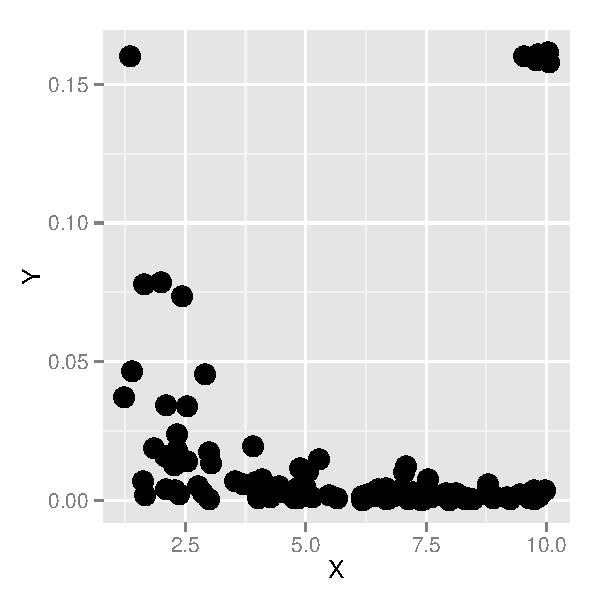
\includegraphics[scale=0.55]{data3.pdf}
%\label{nbin3_a}
%}
%\subfigure[]{
%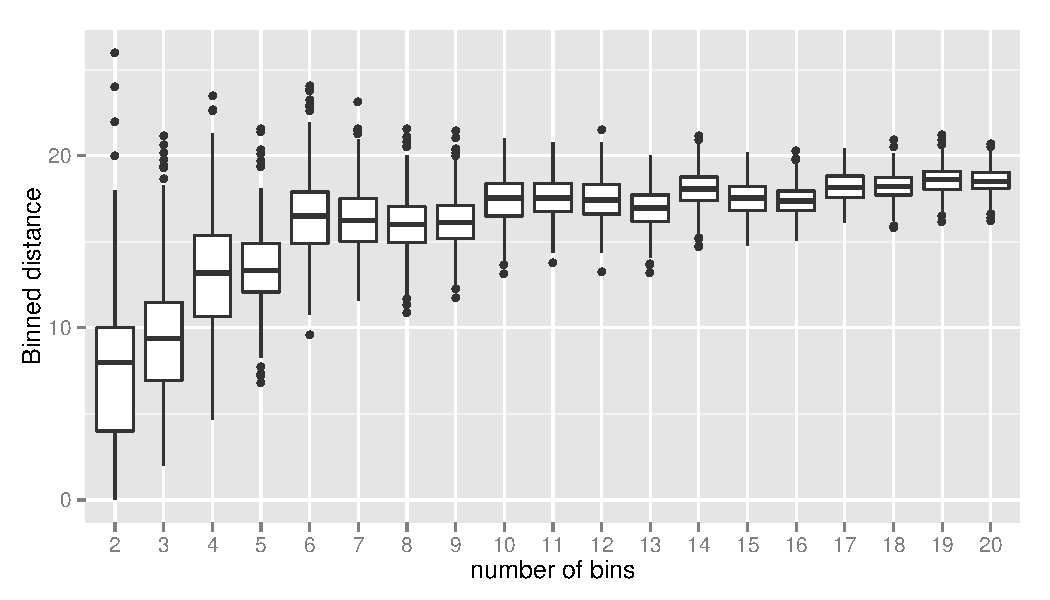
\includegraphics[scale=0.55]{data3-nbin.pdf}
%\label{nbin3_b}
%}
%\label{nbin3}
%	\vspace{-.1in}
%\caption[Optional caption for list of figures]{(a) Plot showing the observed data (b) Binned distance plotted against the number of bins. }
%%{Caption of subfigures \subref{fig:subfig1}, \subref{fig:subfig2} and \subref{fig:subfig3}}
%\end{figure*}

\begin{table*}[hbtp]
\caption{Preferable number of bins for different types of observed data to calculate the binned distance.}
\centering 
\begin{tabular}{p{1.5cm}l c  p{2cm} c cc l c p{4cm}} 
\hline
 Type of Data & Observed Plot && Null Generating Mechanism & A typical null plot && & Difference && (x-bin, y-bin, Max; Min) \\ %[0.5ex] % inserts table %heading 
%\hline
% Linear association & \begin{minipage}[h]{1.5cm} \begin{center} \scalebox{0.25}{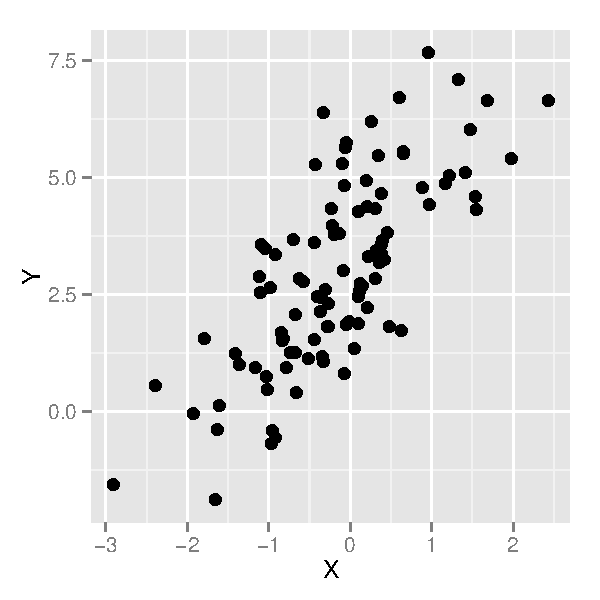
\includegraphics{bin-select-data1.pdf}} \end{center} \end{minipage} && Permutation &  \begin{minipage}[h]{1.5cm} \begin{center} \scalebox{0.25}{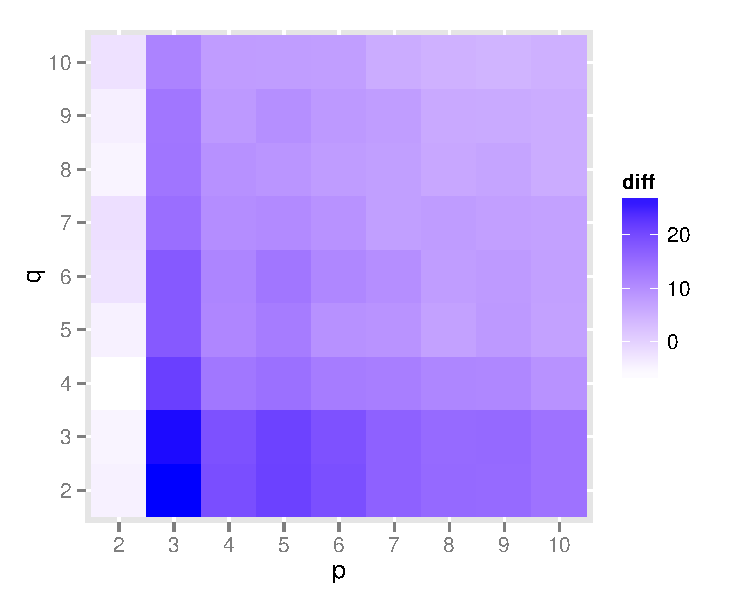
\includegraphics{bin-select-plot1.pdf}} \end{center} \end{minipage} &  \begin{minipage}[h]{1.5cm} \begin{center} \scalebox{0.25}{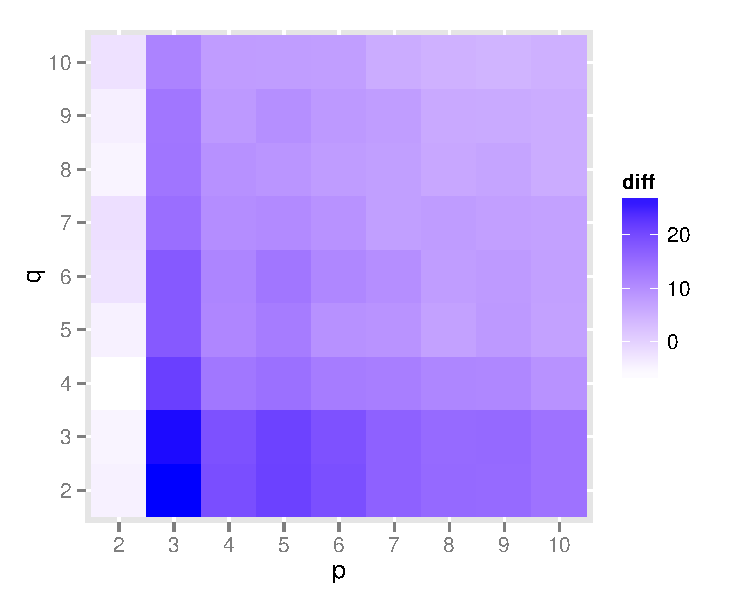
\includegraphics{bin-select-plot1.pdf}} \end{center} \end{minipage} &&           \hspace{0.8cm} small\\
 \hline
 Linear association & \begin{minipage}[h]{1.5cm} \begin{center} \scalebox{0.25}{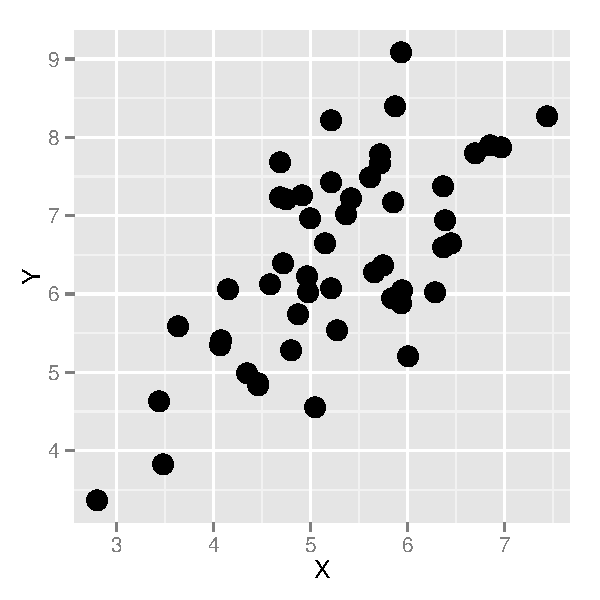
\includegraphics{anscombe-1.pdf}} \end{center} \end{minipage} && Permutation &  \begin{minipage}[h]{1.5cm} \begin{center} \scalebox{0.25}{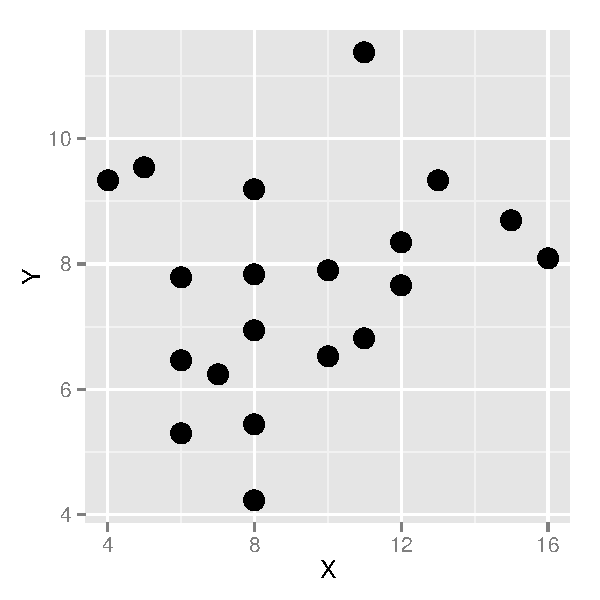
\includegraphics{anscombe-null-1.pdf}} \end{center} \end{minipage} &&&  \begin{minipage}[h]{1.5cm} \begin{center} \scalebox{0.25}{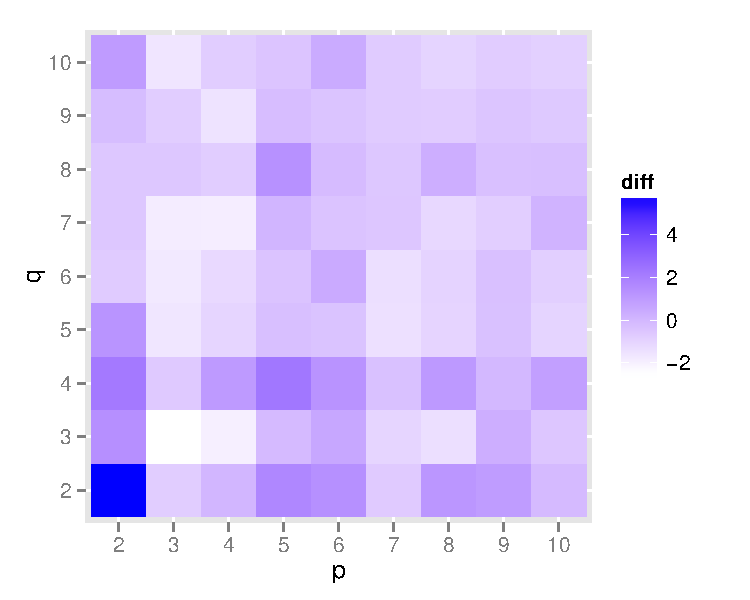
\includegraphics{anscombe-nbin-1.pdf}} \end{center} \end{minipage} &&           \hspace{0.8cm} (2, 2, 5.7 ; - 2.5)\\
 \hline
Nonlinear relationship & \begin{minipage}[h]{1.5cm} \begin{center} \scalebox{0.25}{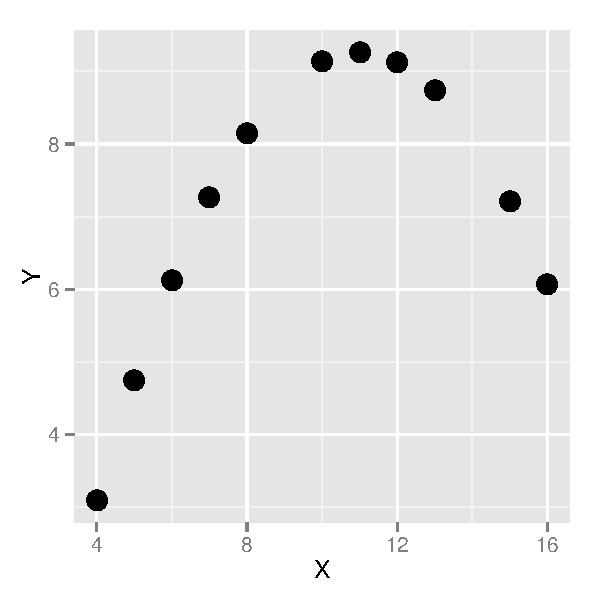
\includegraphics{anscombe-2.pdf}} \end{center} \end{minipage} && Permutation &  \begin{minipage}[h]{1.5cm} \begin{center} \scalebox{0.25}{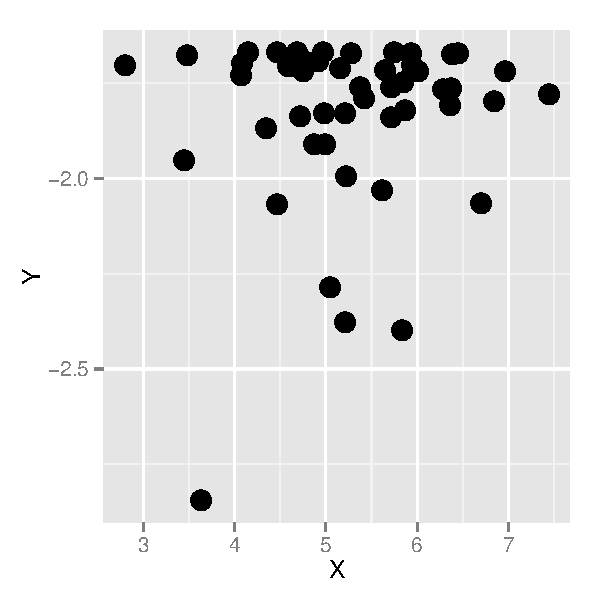
\includegraphics{anscombe-null-2.pdf}} \end{center} \end{minipage} &&&  \begin{minipage}[h]{1.5cm} \begin{center} \scalebox{0.25}{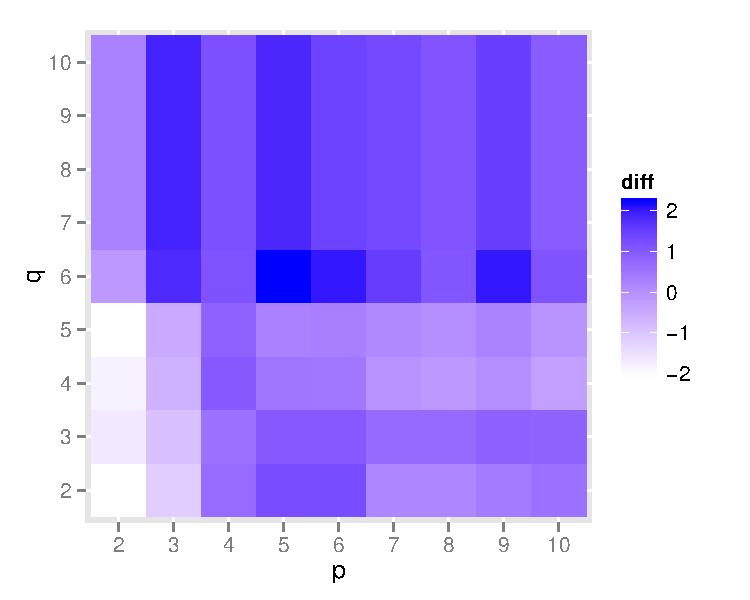
\includegraphics{anscombe-nbin-2.pdf}} \end{center} \end{minipage} &&           \hspace{0.8cm} (2, 10, 6.2 ; - 0.0)\\
 \hline
 Linear relation with outliers & \begin{minipage}[h]{1.5cm} \begin{center} \scalebox{0.25}{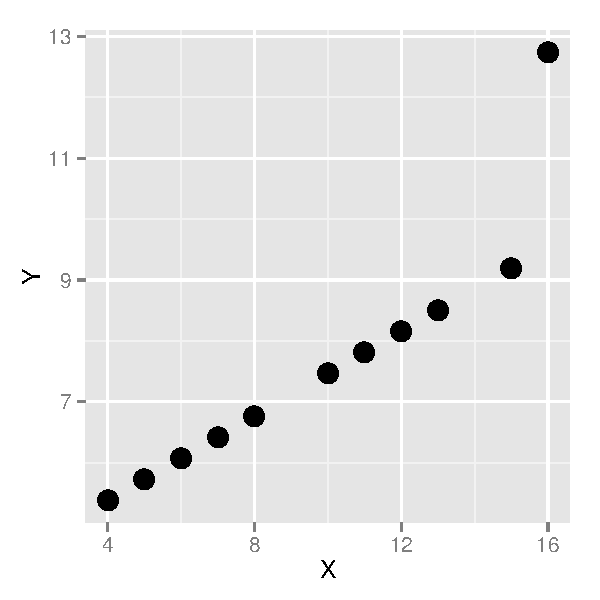
\includegraphics{anscombe-3.pdf}} \end{center} \end{minipage} && Permutation &  \begin{minipage}[h]{1.5cm} \begin{center} \scalebox{0.25}{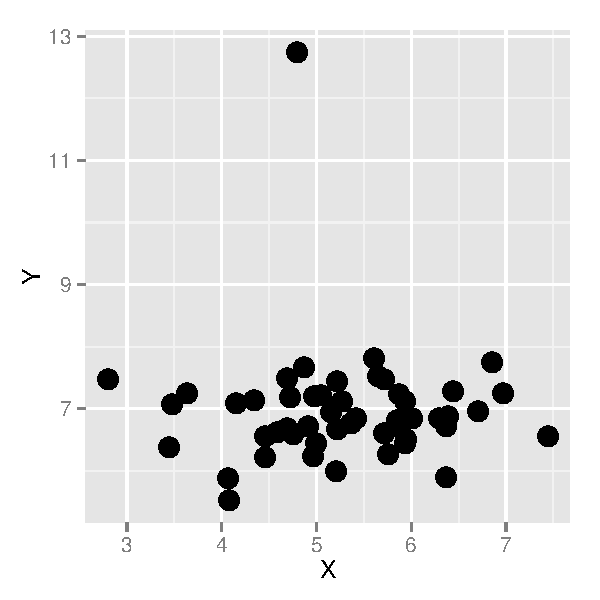
\includegraphics{anscombe-null-3.pdf}} \end{center} \end{minipage} &&&  \begin{minipage}[h]{1.5cm} \begin{center} \scalebox{0.25}{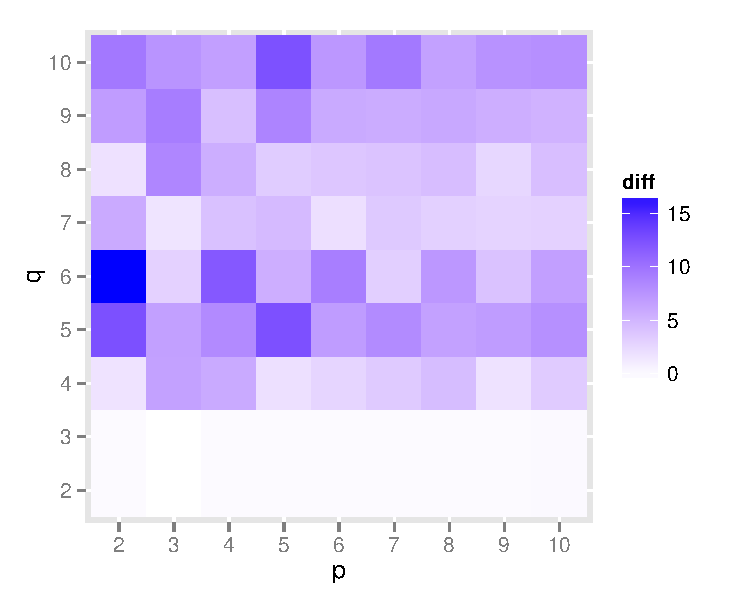
\includegraphics{anscombe-nbin-3.pdf}} \end{center} \end{minipage} &&           \hspace{0.8cm} (2, 6, 16.7 ; - 0.4)\\
 \hline
 Same values with one outlier & \begin{minipage}[h]{1.5cm} \begin{center} \scalebox{0.25}{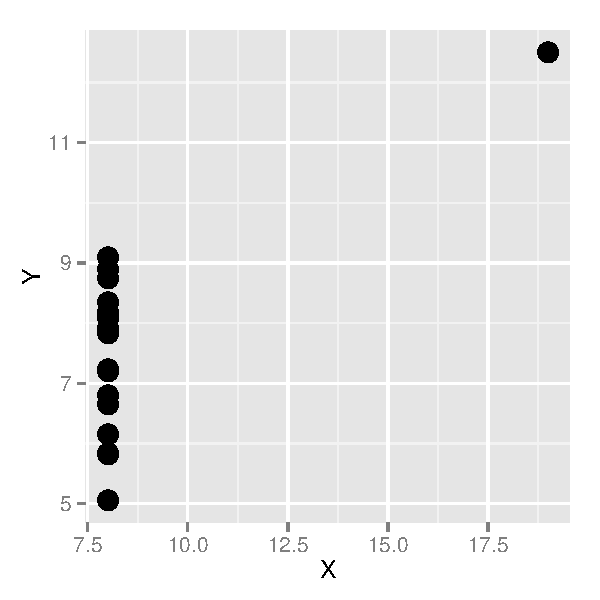
\includegraphics{anscombe-4.pdf}} \end{center} \end{minipage} && Simulation from a \emph{Poi(9)} distribution &  \begin{minipage}[h]{1.5cm} \begin{center} \scalebox{0.25}{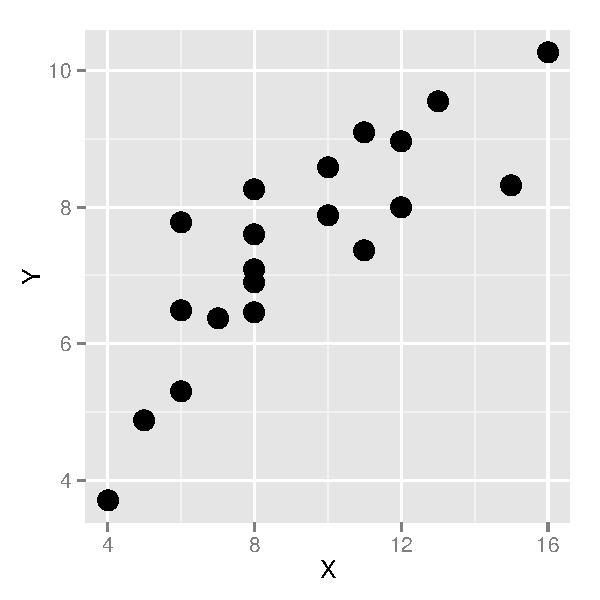
\includegraphics{anscombe-null-4.pdf}} \end{center} \end{minipage} &&&  \begin{minipage}[h]{1.5cm} \begin{center} \scalebox{0.25}{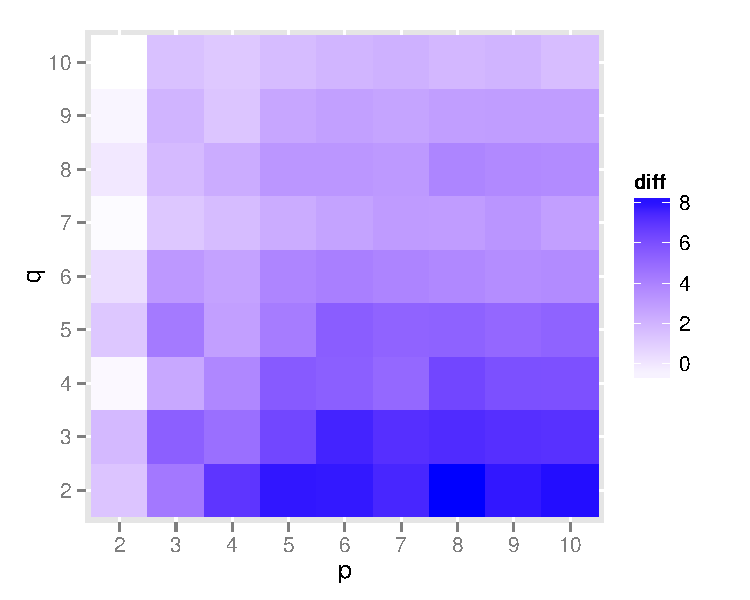
\includegraphics{anscombe-nbin-4.pdf}} \end{center} \end{minipage} &&           \hspace{0.8cm}(10, 3, 34.3 ; - 0.1)\\
 \hline
    Clusters & \begin{minipage}[h]{1.5cm} \begin{center} \scalebox{0.25}{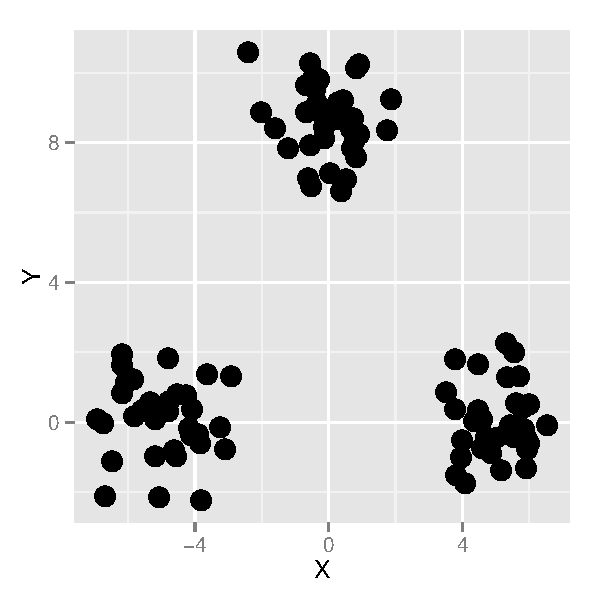
\includegraphics{data1.pdf}} \end{center} \end{minipage} && Permutation &  \begin{minipage}[h]{1.5cm} \begin{center} \scalebox{0.25}{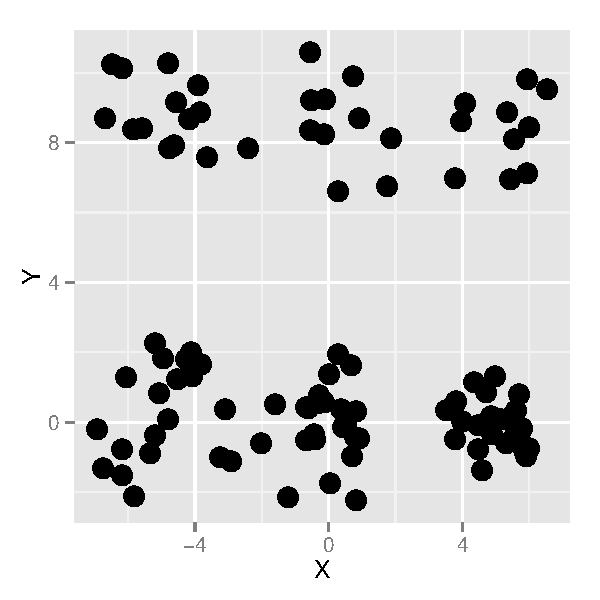
\includegraphics{null1.pdf}} \end{center} \end{minipage} &&&  \begin{minipage}[h]{1.5cm} \begin{center} \scalebox{0.25}{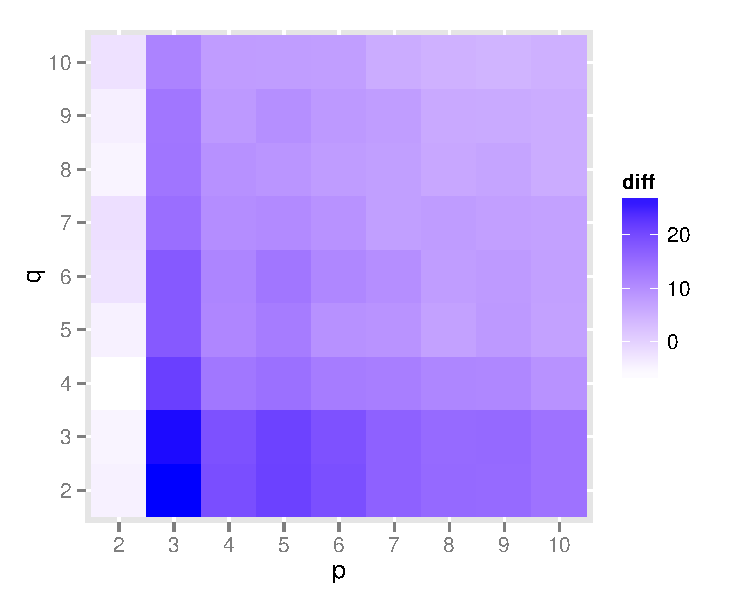
\includegraphics{bin-select-plot1.pdf}} \end{center} \end{minipage} &&           \hspace{0.8cm} (3, 2, 27.6 ; - 5.7)\\
 \hline
%Clusters & \begin{minipage}[h]{1.5cm} \begin{center} \scalebox{0.25}{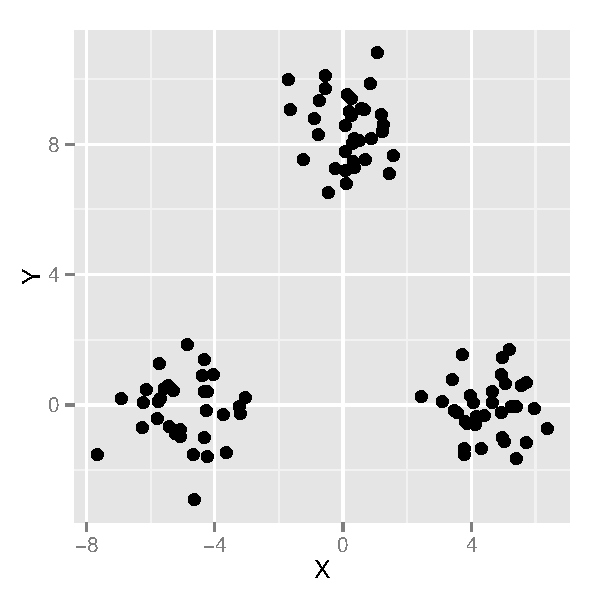
\includegraphics{bin-select-data2.pdf}} \end{center} \end{minipage} && Permutation &  \begin{minipage}[h]{1.5cm} \begin{center} \scalebox{0.25}{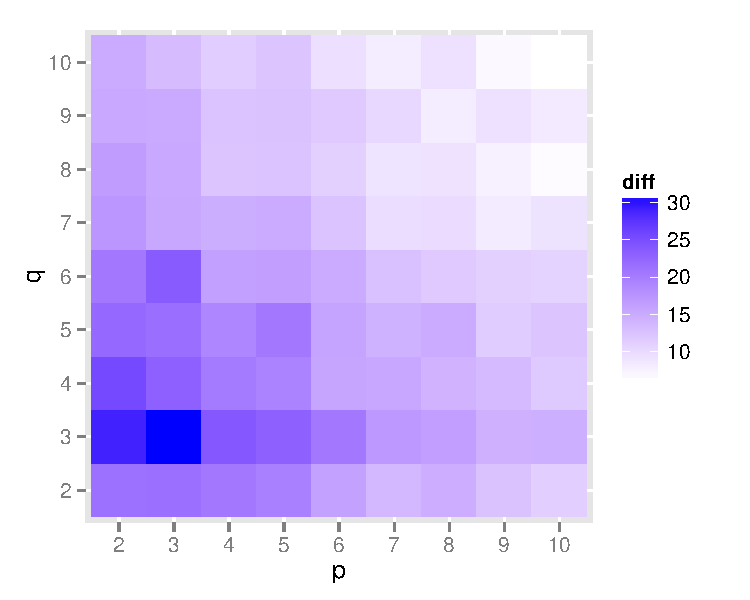
\includegraphics{bin-select-plot2.pdf}} \end{center} \end{minipage} && \hspace{0.8cm} small\\
% \hline
% Discrete vs. Continuous & \begin{minipage}[h]{1.5cm} \begin{center} \scalebox{0.25}{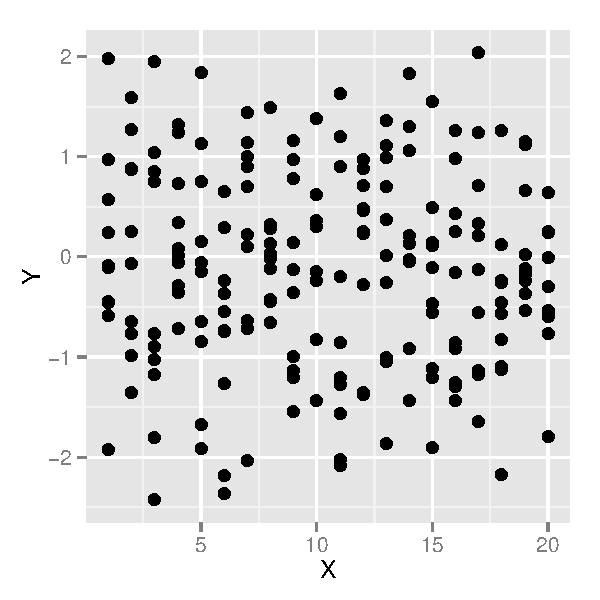
\includegraphics{bin-select-data3.pdf}} \end{center} \end{minipage} && Simulation from a specific distribution &  \begin{minipage}[h]{1.5cm} \begin{center} \scalebox{0.25}{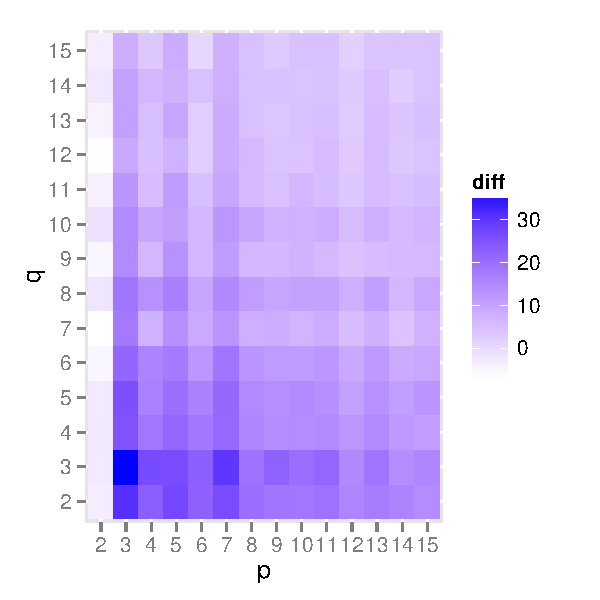
\includegraphics{bin-select-plot3.pdf}} \end{center} \end{minipage} && \hspace{0.8cm} small\\
% \hline
% Discrete vs. Continuous & \begin{minipage}[h]{1.5cm} \begin{center} \scalebox{0.25}{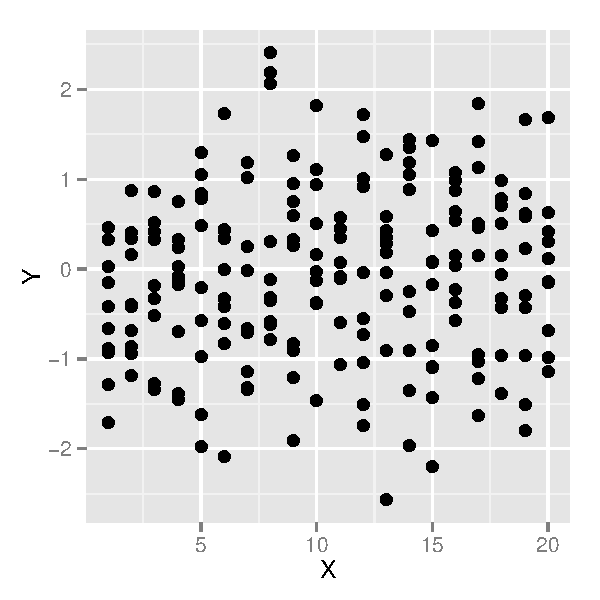
\includegraphics{bin-select-data4.pdf}} \end{center} \end{minipage} && Permutation &  \begin{minipage}[h]{1.5cm} \begin{center} \scalebox{0.25}{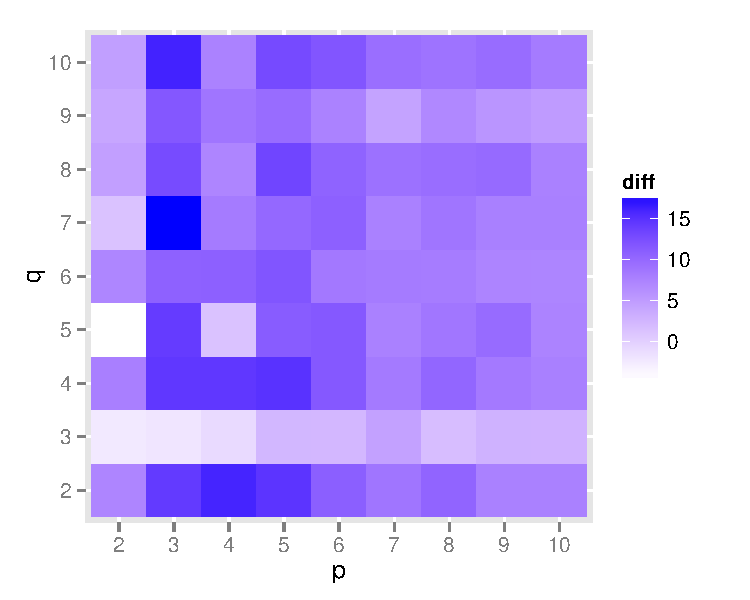
\includegraphics{bin-select-plot4.pdf}} \end{center} \end{minipage} && \hspace{0.8cm} large\\
% \hline
%Presence of Outlier(s) & \begin{minipage}[h]{1.5cm} \begin{center} \scalebox{0.25}{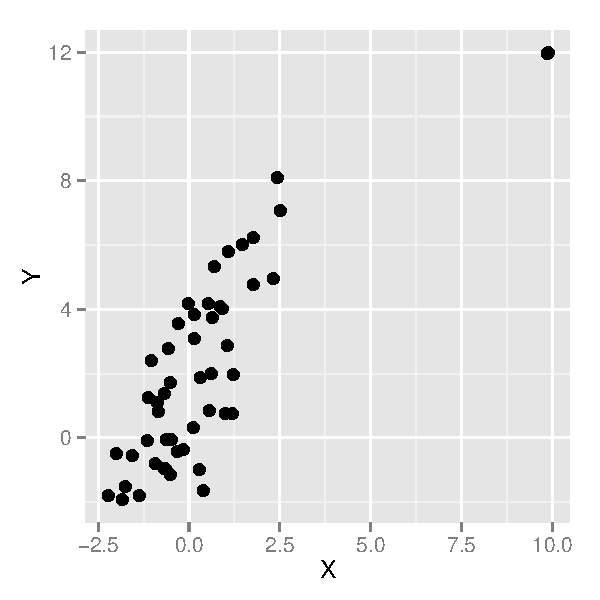
\includegraphics{bin-select-data5.pdf}} \end{center} \end{minipage} && Simulation from a specific distribution &  \begin{minipage}[h]{1.5cm} \begin{center} \scalebox{0.25}{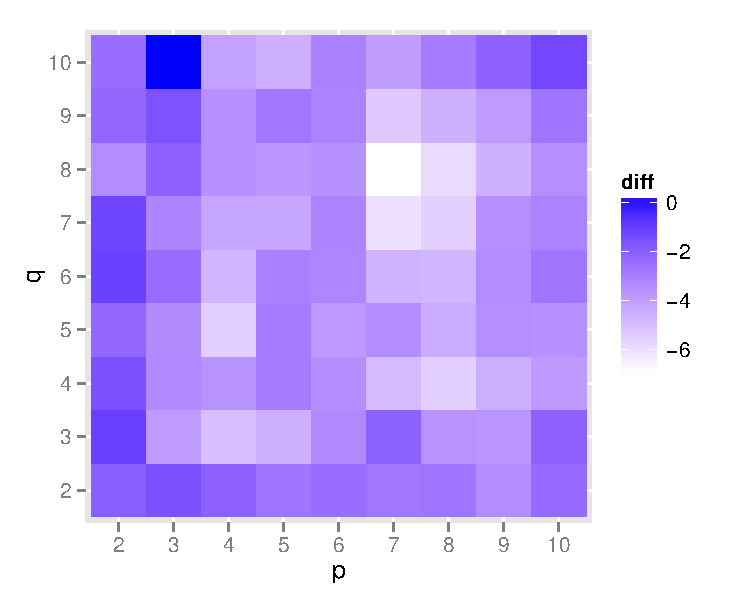
\includegraphics{bin-select-plot5.pdf}} \end{center} \end{minipage} && \hspace{0.8cm} small\\
% \hline
\end{tabular}
\label{tbl:bin1}
\end{table*}

%\newpage
\begin{table*}[hbtp]
\caption{Preferable number of bins for different types of observed data to calculate the binned distance.}
\centering 
\begin{tabular}{p{1.5cm}l c  p{2cm} c cc l c p{4cm}} 
\hline
 Type of Data & Observed Plot && Null Generating Mechanism & A typical null plot && & Difference && (x-bin, y-bin, Max; Min) \\ %[0.5ex] % inserts table %heading 
 \hline
Categorical & \begin{minipage}[h]{1.5cm} \begin{center} \scalebox{0.25}{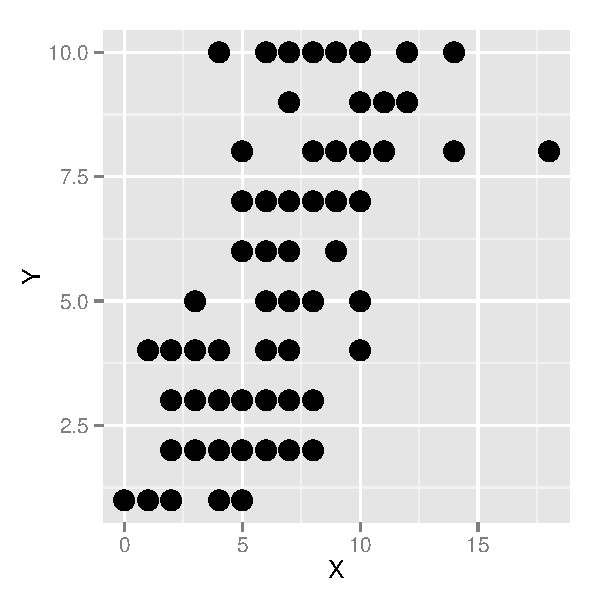
\includegraphics{data2.pdf}} \end{center} \end{minipage} && Simulation from a Normal distribution &  \begin{minipage}[h]{1.5cm} \begin{center} \scalebox{0.25}{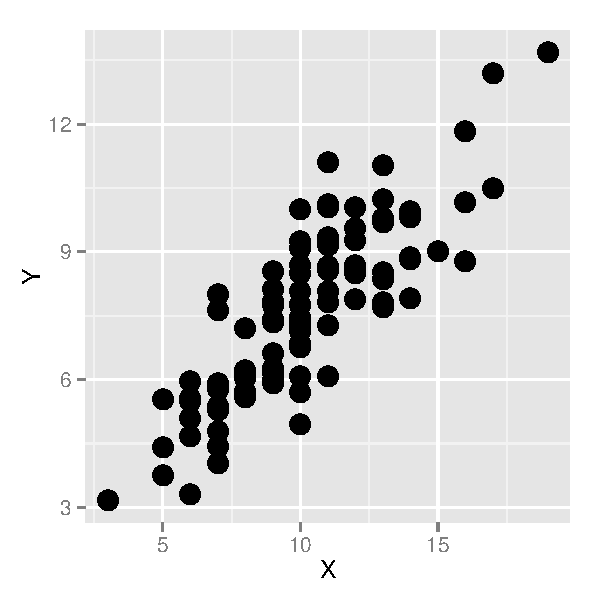
\includegraphics{null2.pdf}} \end{center} \end{minipage} &&&  \begin{minipage}[h]{1.5cm} \begin{center} \scalebox{0.25}{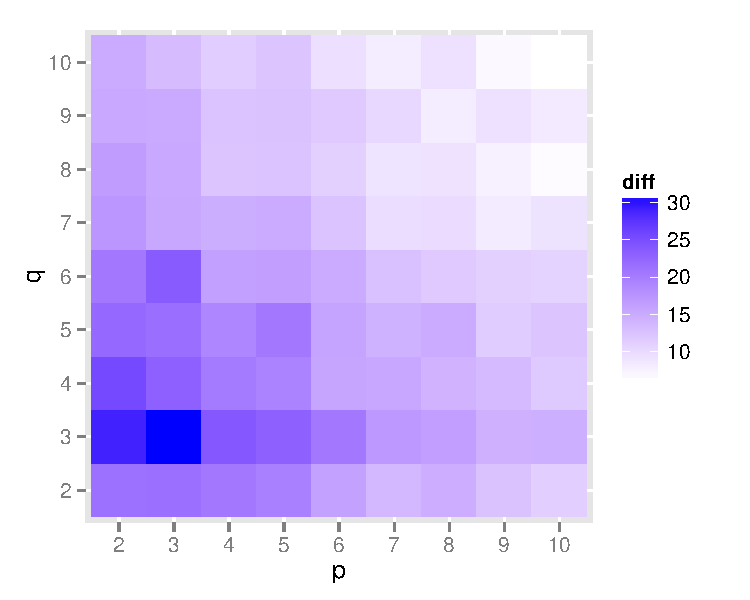
\includegraphics{bin-select-plot2.pdf}} \end{center} \end{minipage} &&           \hspace{0.8cm} (3, 3, 30.7; 6.2) \\
 \hline
Nonlinear relation with outliers & \begin{minipage}[h]{1.5cm} \begin{center} \scalebox{0.25}{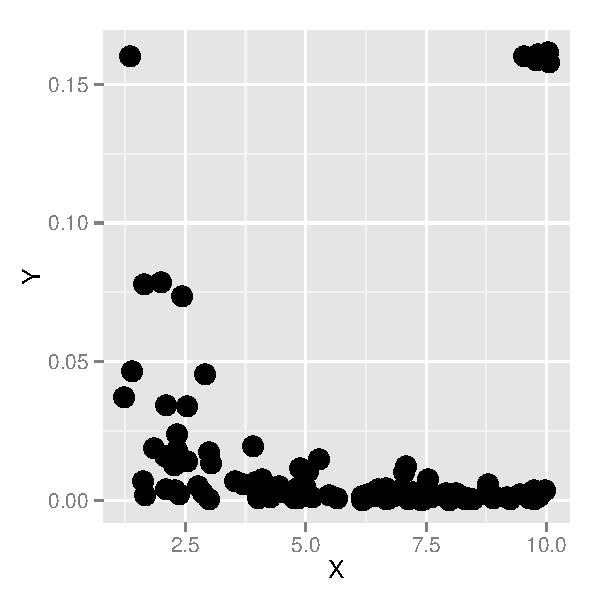
\includegraphics{data3.pdf}} \end{center} \end{minipage} && Permutation &  \begin{minipage}[h]{1.5cm} \begin{center} \scalebox{0.25}{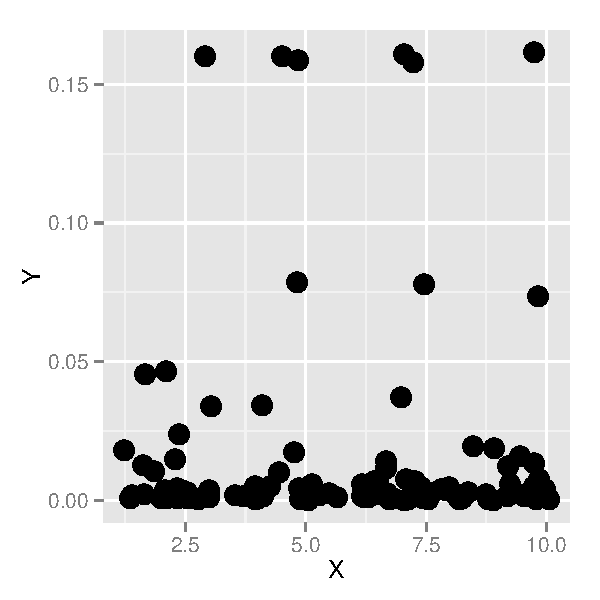
\includegraphics{null3.pdf}} \end{center} \end{minipage} &&&  \begin{minipage}[h]{1.5cm} \begin{center} \scalebox{0.25}{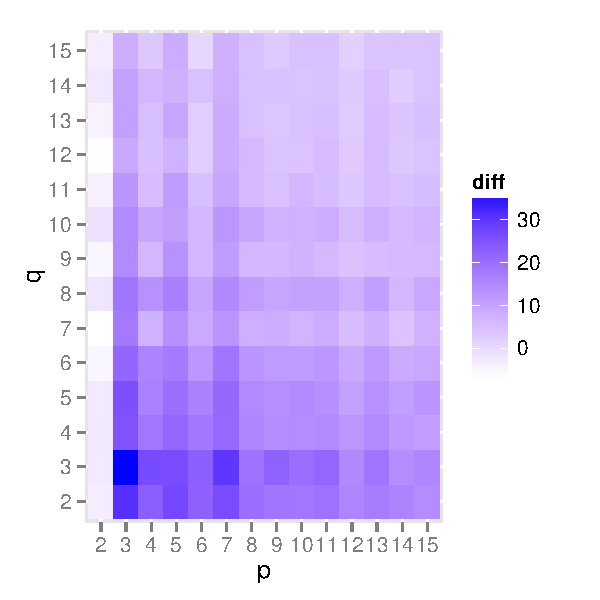
\includegraphics{bin-select-plot3.pdf}} \end{center} \end{minipage} &&           \hspace{0.8cm} (4, 10, 3.9; -3.4) \\
 \hline
Linear relationship with outlier  & \begin{minipage}[h]{1.5cm} \begin{center} \scalebox{0.25}{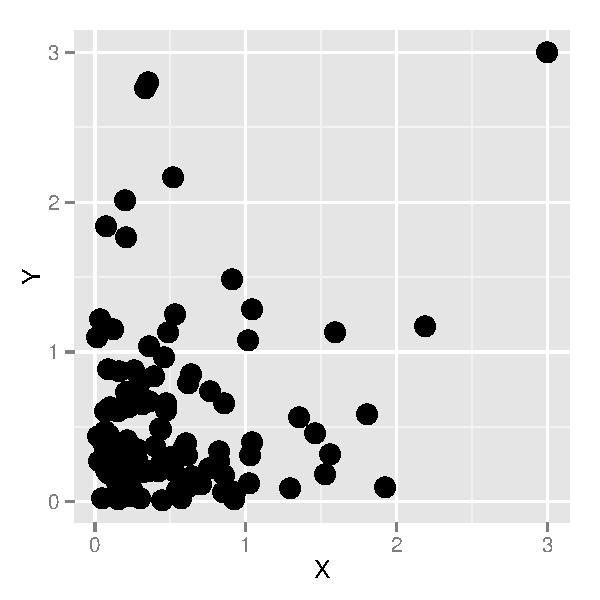
\includegraphics{data5.pdf}} \end{center} \end{minipage} && Permutation &  \begin{minipage}[h]{1.5cm} \begin{center} \scalebox{0.25}{\includegraphics{null5.pdf}} \end{center} \end{minipage} &&&  \begin{minipage}[h]{1.5cm} \begin{center} \scalebox{0.25}{\includegraphics{bin-select-plot5.pdf}} \end{center} \end{minipage} &&           \hspace{0.8cm} (3, 10, 0.3; -7.1) \\
 \hline
 Residual Plot & \begin{minipage}[h]{1.5cm} \begin{center} \scalebox{0.25}{\includegraphics{data4.pdf}} \end{center} \end{minipage} && Simulation from the null model &  \begin{minipage}[h]{1.5cm} \begin{center} \scalebox{0.25}{\includegraphics{null4.pdf}} \end{center} \end{minipage} &&&  \begin{minipage}[h]{1.5cm} \begin{center} \scalebox{0.25}{\includegraphics{bin-select-plot4.pdf}} \end{center} \end{minipage} &&           \hspace{0.8cm} (3, 7, 17.8; -4.5)\\
 \hline
 Residual Plot & \begin{minipage}[h]{1.5cm} \begin{center} \scalebox{0.25}{\includegraphics{data6.pdf}} \end{center} \end{minipage} && Simulation from the null model &  \begin{minipage}[h]{1.5cm} \begin{center} \scalebox{0.25}{\includegraphics{null6.pdf}} \end{center} \end{minipage} &&&  \begin{minipage}[h]{1.5cm} \begin{center} \scalebox{0.25}{\includegraphics{bin-select-plot6.pdf}} \end{center} \end{minipage} &&           \hspace{0.8cm} (2, 5, 4.8; -4.4)\\
 \hline
Spiral data & \begin{minipage}[h]{1.5cm} \begin{center} \scalebox{0.25}{\includegraphics{data7.pdf}} \end{center} \end{minipage} && Permutation &  \begin{minipage}[h]{1.5cm} \begin{center} \scalebox{0.25}{\includegraphics{null7.pdf}} \end{center} \end{minipage} &&&  \begin{minipage}[h]{1.5cm} \begin{center} \scalebox{0.25}{\includegraphics{bin-select-plot7.pdf}} \end{center} \end{minipage} &&           \hspace{0.8cm} (5, 7, 23.6; -11.9)\\
 \hline
Contaminated data & \begin{minipage}[h]{1.5cm} \begin{center} \scalebox{0.25}{\includegraphics{data8.pdf}} \end{center} \end{minipage} && Permutation &  \begin{minipage}[h]{1.5cm} \begin{center} \scalebox{0.25}{\includegraphics{null8.pdf}} \end{center} \end{minipage} &&&  \begin{minipage}[h]{1.5cm} \begin{center} \scalebox{0.25}{\includegraphics{bin-select-plot8.pdf}} \end{center} \end{minipage} &&           \hspace{0.8cm} (5, 3, 8.1; -2.5)\\
 \hline
%Clusters & \begin{minipage}[h]{1.5cm} \begin{center} \scalebox{0.25}{\includegraphics{bin-select-data2.pdf}} \end{center} \end{minipage} && Permutation &  \begin{minipage}[h]{1.5cm} \begin{center} \scalebox{0.25}{\includegraphics{bin-select-plot2.pdf}} \end{center} \end{minipage} && \hspace{0.8cm} small\\
% \hline
% Discrete vs. Continuous & \begin{minipage}[h]{1.5cm} \begin{center} \scalebox{0.25}{\includegraphics{bin-select-data3.pdf}} \end{center} \end{minipage} && Simulation from a specific distribution &  \begin{minipage}[h]{1.5cm} \begin{center} \scalebox{0.25}{\includegraphics{bin-select-plot3.pdf}} \end{center} \end{minipage} && \hspace{0.8cm} small\\
% \hline
% Discrete vs. Continuous & \begin{minipage}[h]{1.5cm} \begin{center} \scalebox{0.25}{\includegraphics{bin-select-data4.pdf}} \end{center} \end{minipage} && Permutation &  \begin{minipage}[h]{1.5cm} \begin{center} \scalebox{0.25}{\includegraphics{bin-select-plot4.pdf}} \end{center} \end{minipage} && \hspace{0.8cm} large\\
% \hline
%Presence of Outlier(s) & \begin{minipage}[h]{1.5cm} \begin{center} \scalebox{0.25}{\includegraphics{bin-select-data5.pdf}} \end{center} \end{minipage} && Simulation from a specific distribution &  \begin{minipage}[h]{1.5cm} \begin{center} \scalebox{0.25}{\includegraphics{bin-select-plot5.pdf}} \end{center} \end{minipage} && \hspace{0.8cm} small\\
% \hline
\end{tabular}
\label{tbl:bin2}
\end{table*}

The rationale behind selecting different types of data is to investigate how the optimal number of bins or bin sizes varies with different types of data. The different null generating mechanisms are also selected for the same reason. In Table \ref{tbl:bin1} the first four observed data plots corresponds to the datasets described by Francis Anscombe in \citep{anscombe:1972} but with large number of data points. Although the datasets have the same pattern, the datasets do not follow the properties of Anscombe's quartet. The fifth dataset is a data with 3 distinct clusters. In Table \ref{tbl:bin2}, the first dataset shows a categorical data. The second and the third data are non-linear and linear association with the presence of outliers. The fourth and fifth datasets are the residual plots with curved pattern and non-constant variance pattern. The sixth data is a spiral data while the seventh one is a data with contamination. 

The differences, $\delta_{\hbox{lineup}}$, are represented in a tile plot where each tile gives the difference for each combination. The dark blue shows higher values while the white shows lower values. It can be seen that the plots look different for the different datasets. Hence the optimal number of bins varies from data to data. No specific pattern is evident in the plot. But overall it can be seen that for strong linear relationship, small number of bins should be preferred over large number of bins. Also when outlier is present in the data, larger number of bins is preferred at least in one axis.

It is important to mention at this point that Table \ref{tbl:bin1} and Table \ref{tbl:bin2} is not meant to provide any guidelines for the selection of number of bins. The Tables only show that the binned distance is highly affected by the number of bins and the type of data. It is advisable to find the optimal number of bins for a given data before using the binned distance.


\section{Results} \label{sec:results}

%{\color{blue} Description of the Turk Results and analysis.}

The performance of the distance metrics was evaluated with comparing the distances with the response of the subjects. A number of experiments were done in Amazon Mechanical Turk \citep{turk}. Subjects were recruited through Amazon Mechanical Turk \citep{turk} and were shown a sequence of lineups. In each experiment, they were asked specific questions. Their responses were recorded along with other demographic informations. The details about the design of experiments can be found in \cite{majumder:2011} and \cite{roychowdhury:2013}. 

\subsection{Turk Experiment -- Side by Side Boxplots}

In this experiment, all the lineups generated had a side by side boxplot as the test statistic. Assuming that the null hypothesis is true, the null plots were generated by assuming that there is no difference between the two distributions. The subjects were shown a few lineups and were asked to identify the plot which has the largest vertical difference between group 1 and group 2. Figure \ref{turk1} gives such a lineup. \\

\begin{figure}[htbp]
\centering
\includegraphics[width=.5\textwidth]{turk1-example.pdf}
%\includegraphics[width=.65\textwidth]{large-p-trim-bin.pdf}
\caption{An example lineup from Turk Experiment 1. The lineup has $m = 20$ plots of which one is the observed data plot and the remaining $m - 1$ are the null plots generated assuming that the null hypothesis is true. Subjects were asked to identify the plot which has the largest vertical difference between the two groups. Can you identify the observed plot ?}
\label{turk1}
\end{figure}

The response of the subjects were noted and the proportion of correct response was calculated for each lineup. The distances between the plots in each lineup were computed using both the distance based on boxplots ($d_{\hbox{box}}$) and the binned distance ($d_{\hbox{bin}}$). The mean distance for the true plot and the null plots were calculated and $\delta_{\hbox{lineup}}$ and $\gamma_{\hbox{lineup}}$ are obtained. The proportion of correct response was plotted against each of the two statistics. Figure \ref{turk1comp} (a) - (b) shows the proportion correct against the difference for $d_{\hbox{box}}$ and $d_{\hbox{bin}}$ respectively. Figure \ref{turk1comp} (c) - (d) shows the proportion correct against the number of null plots greater than the observed plot for the two distance measures respectively. 


\begin{figure}[hbtp]
\centering
\subfigure[]{
\includegraphics[scale=0.55]{turk1-diff-box-prop.pdf}
\label{t1comp_1}
}
\subfigure[]{
\includegraphics[scale=0.55]{turk1-diff-bin-prop-8.pdf}
\label{t1bin_1}
}
\subfigure[]{
\includegraphics[scale=0.55]{turk1-grtr-box-prop.pdf}
\label{t1comp_2}
}
\subfigure[]{
\includegraphics[scale=0.55]{turk1-grtr-bin-prop-8.pdf}
\label{t1bin_2}
}
\label{turk1comp}
	\vspace{-.1in}
\caption[Optional caption for list of figures]{(a) Plot showing the proportion correct against the difference based on the boxplot distance and (b) based on the binned distance. In both figures the vertical line represents the difference equal to 0 when there is at least one null plot similar to the observed plot. The proportion correct increases with the difference. (c) Plot showing the proportion correct against the number of null plots greater than the observed plot according to the boxplot distance and (d) according to the binned distance. The proportion correct decreases as the number of null plots greater than the observed plot increases.  }
%{Caption of subfigures \subref{fig:subfig1}, \subref{fig:subfig2} and \subref{fig:subfig3}}
\end{figure}

%\newpage

In Figure \ref{turk1comp} (a) - (b), the proportion correct is plotted against the difference. The red vertical line represents difference equal to 0 indicating that the mean distance of the true plot is equal to the maximum of the mean distance of the null plots i.e. the mean distance of the true plot is equal to at least one of the mean distance of the null plots. It can be seen that as the difference increases, the proportion correct increases. So the subjects do better in the easier lineups than the hard ones. The binned distance was calculated using 8 bins on both the axes.

Figure \ref{turk1comp} (c) - (d) shows the relation between proportion correct and the number of null plots larger than the true plot. It can be seen that as there are more extreme null plots compared to the observed plot, the subjects find it difficult to pick the observed plot. It is interesting to see that the subjects can pick the observed plot with one or two extreme null plots. 

Though the distance based on the boxplots works better, the binned distance does a decent job in this case. According to the binned distance, there are a few lineups which has a negative difference but the proportion correct is above 60\%, which can be also be seen in Figure \ref{turk1comp} (d). It should be noted that the binned distance does not take into account the graphical elements of the plot (e.g. boxplot) and calculates the distance solely based on the data. So an outlier may have a huge effect on the binned distance but does not effect the distance based on the boxplots. Hence it is advisable to use a distance based on the graphical elements since that is exactly what the subjects look at in the lineup.

The time taken to respond by the subjects is another measure of difficulty of the lineups. Due the presence of some huge outliers, the median time taken by the subjects for each lineup is looked at and plotted against the difference for both the distance measures. Figure \ref{turk1-mtime} shows the plots. It can be clearly seen that when the difference is below 0, there is no real trend in the median time and there is a huge variability, indicating that the time taken depends on the subjects. But when the difference is above 0, the median time decreases rapidly as the difference increases. Hence the subjects can pick the true plot quickly if the true plot is extreme compared to the null plots.
 
%\begin{figure}[hbtp]
%\centering
%\subfigure[]{
%\includegraphics[scale=0.55]{turk1-diff-bin-prop-8.pdf}
%\label{t1bin_1}
%}
%\subfigure[]{
%\includegraphics[scale=0.55]{turk1-grtr-bin-prop-8.pdf}
%\label{t1bin_2}
%}
%%\label{turk1-bin}
%	\vspace{-.1in}
%\caption[Optional caption for list of figures]{(a) Plot showing the proportion correct against the difference based on the binned distance with 8 bins on each axis. The vertical line represents the difference equal to 0 when there is at least one null plot similar to the observed plot. The proportion correct increases with the difference. (b) Plot showing the proportion correct against the number of null plots greater than the observed plot according to the binned distance. The proportion correct decreases as the number of null plots greater than the observed plot increases.  }
%%{Caption of subfigures \subref{fig:subfig1}, \subref{fig:subfig2} and \subref{fig:subfig3}}
%\end{figure}

\begin{figure}[hbtp]
\centering
\subfigure[]{
\includegraphics[scale=0.55]{turk1-diff-box-mtime.pdf}
\label{t1comp_1}
}
\subfigure[]{
\includegraphics[scale=0.55]{turk1-diff-bin-mtime.pdf}
\label{t1bin_1}
}
\label{turk1-mtime}
	\vspace{-.1in}
\caption[Optional caption for list of figures]{Plot showing the median time to respond by the subjects against the difference based on the boxplot distance in (a) and binned distance in (b). In both the plots, the vertical line represents the difference equal to 0 when there is at least one null plot similar to the observed plot. The median time decreases with the difference.  }
%{Caption of subfigures \subref{fig:subfig1}, \subref{fig:subfig2} and \subref{fig:subfig3}}
\end{figure}


\subsection{Turk Experiment -- Scatterplots with a regression line overlaid}

In this experiment, the test statistic is a scatterplot with the regression line overlaid. Assuming that the null hypothesis is true, the null plots are generated by assuming that there is no significant linear relationship between the two variables. The subjects were shown a few lineups and were asked to identify the plot which has the steepest slope. Figure \ref{turk2} gives such a lineup. 

\begin{figure}[htbp]
\centering
\includegraphics[width=.5\textwidth]{turk2-example.pdf}
%\includegraphics[width=.65\textwidth]{large-p-trim-bin.pdf}
\caption{An example lineup from Turk Experiment 2. In this lineup, one of the plots is the observed plot and the other 19 plots are the null plots generated assuming that the null hypothesis $H_o : \beta = 0$ is true. Subjects were asked to identify the plot with the steepest slope. Can you identify the observed plot ?}
\label{turk2}
\end{figure}

The distances between the plots in this experiment were computed using both the distance based on regression line ($d_{\hbox{reg}}$) and the binned distance ($d_{\hbox{bin}}$) with a small number of bins. The proportion of correct response for each lineup was calculated from the response of the subjects and plotted against $\delta_{\hbox{lineup}}$ and $\gamma_{\hbox{lineup}}$.  Figure \ref{turk2comp}(a), (b) shows the results for the distance based on the regression line and the binned distance against $\delta_{\hbox{lineup}}$.


\begin{figure*}[hbtp]
\centering
\subfigure[]{
\includegraphics[scale=0.55]{turk2-diff-reg-prop.pdf}
\label{t2comp_1}
}
\subfigure[]{
\includegraphics[scale=0.55]{turk2-diff-bin-prop-2.pdf}
\label{t2comp_2}
}
\subfigure[]{
\includegraphics[scale=0.55]{turk2-grtr-reg-prop.pdf}
\label{t2comp_1}
}
\subfigure[]{
\includegraphics[scale=0.55]{turk2-grtr-bin-prop-2.pdf}
\label{t2comp_2}
}
\label{turk2comp}
	\vspace{-.1in}
\caption[Optional caption for list of figures]{(a) Plot showing the proportion correct against the difference based on the regression distance and (b) based on the binned distance. In both figures the vertical line represents the difference equal to 0 when there is at least one null plot similar to the observed plot. The proportion correct increases with the difference. (c) Plot showing the proportion correct against the number of null plots greater than the observed plot according to the regression distance and (d) according to the binned distance. The proportion correct decreases as the number of null plots greater than the observed plot increases.}
%{Caption of subfigures \subref{fig:subfig1}, \subref{fig:subfig2} and \subref{fig:subfig3}}
\end{figure*}

Figure \ref{turk2comp}(a) - (b) shows the proportion correct against the difference. The vertical line represents difference equal to 0. It can be seen that as the difference increases, the proportion correct increases. So the subjects do better in the easier lineups than the hard ones. The distance based on regression works well in capturing the complexity of the lineups. But the binned distance fails to do so. Although the proportion correct increases with difference, the proportion correct is high for values with negative difference. This is a classic case where a graphical element affects the response. The presence of the overlaid regression line on almost transparent points of the scatterplot mattered in the subjects picking the correct plot. One other reason may be the use of the same number of bins (2 $\times$ 2) in this case for all the lineups. 

Figure \ref{turk2comp} (c) - (d) shows that as there are more extreme null plots compared to the observed plot, the subjects find it difficult to pick the observed plot. For a few lineups, almost all the subjects identify the observed plot although there is one more extreme null plot. Though from Figure \ref{turk2comp}, it can be seen that the extremeness is marginal in most cases. 

\begin{figure}[hbtp]
\centering
\subfigure[]{
\includegraphics[scale=0.55]{turk2-diff-reg-mtime.pdf}
\label{t1comp_1}
}
\subfigure[]{
\includegraphics[scale=0.55]{turk2-diff-bin-mtime.pdf}
\label{t1bin_1}
}
\label{turk2-mtime}
	\vspace{-.1in}
\caption[Optional caption for list of figures]{Plot showing the median time to respond by the subjects against the difference based on the regression distance in (a) and binned distance in (b). In both the plots, the vertical line represents the difference equal to 0 when there is at least one null plot similar to the observed plot. The median time decreases with the difference.  }
%{Caption of subfigures \subref{fig:subfig1}, \subref{fig:subfig2} and \subref{fig:subfig3}}
\end{figure}

Figure \ref{turk2-mtime} shows the relationship between the median time taken to respond and the difference for both the distances. It can be clearly seen that there is a strong negative association showing that as the difference increases, the subjects take lesser time to respond. Also the variability of the median time is higher for smaller difference. In case of binned distance, the relationship is negative though the variability is higher for the above mentioned reasons.

\subsection{Turk Experiment -- Large $p$, Small $n$ data}

The motivation behind this experiment is to study the effect of large dimensions in a data with complete noise and some real separation. Data was simulated with different dimensions and fixed sample size. Data was divided into two or three groups. A projection pursuit with Penalized Discriminant Analysis Index was used and the one and two dimensional projections were obtained. The one or two dimensional projections were then plotted which resulted in the observed data plot. To generate the null data, the group variable in the data was permuted and the projection pursuit was applied. The subjects were shown these lineups and were asked to identify the plot with the most separated colored groups. Figure \ref{largep} gives an example of such a lineup with two dimensional projections with 3 colored groups. 

\begin{figure}[htbp]
\centering
\includegraphics[width=.7\textwidth]{largep-example.pdf}
%\includegraphics[width=.65\textwidth]{large-p-trim-bin.pdf}
\caption{An example lineup from Large $p$, Small $n$ Turk Experiment.}
\label{largep}
\end{figure}

The distances between the plots in this experiment were computed using the distance based on separation of the clusters and the binned distance. The number of bins used for the lineups with one dimensional projections is larger (10 in this case) but for the lineups with two dimensional projections, the number of bins used is 5. The proportion of correct response is plotted against $\delta_{\hbox{lineup}}$ and $\gamma_{\hbox{lineup}}$ for both the distances. Figure \ref{lp-comp} shows the results for the binned distance.


\begin{figure*}[hbtp]
\centering
\subfigure[]{
\includegraphics[scale=0.55]{largep-diff-clus-prop.pdf}
\label{lpcomp_1}
}
\subfigure[]{
\includegraphics[scale=0.55]{largep-diff-bin-prop-10-5.pdf}
\label{lpcomp_2}
}
\subfigure[]{
\includegraphics[scale=0.55]{largep-grtr-bin-prop-10-5.pdf}
\label{lpcomp_1}
}
\subfigure[]{
\includegraphics[scale=0.55]{largep-grtr-clus-prop.pdf}
\label{lpcomp_2}
}
\label{lp-comp}
	\vspace{-.1in}
\caption[Optional caption for list of figures]{(a) Plot showing the proportion correct against the difference based on the separation distance and (b) based on the binned distance. In both figures the vertical line represents the difference equal to 0 when there is at least one null plot similar to the observed plot. The proportion correct increases with the difference. (c) Plot showing the proportion correct against the number of null plots greater than the observed plot according to the separation distance and (d) according to the binned distance. The proportion correct decreases as the number of null plots greater than the observed plot increases.}
%{Caption of subfigures \subref{fig:subfig1}, \subref{fig:subfig2} and \subref{fig:subfig3}}
\end{figure*}

In Figure \ref{lp-comp} (a) - (b), the proportion correct is plotted against the difference for distance based on separation and the binned distance respectively. The red vertical line shows difference equal to 0.  It can be seen that as the difference increases, the proportion correct increases and both the distances do a good job in capturing the response of the subjects. 

Figure \ref{lp-comp}(c) - (d) shows that as there are more extreme null plots compared to the observed plot, the subjects find it difficult to pick the observed plot. For a few lineups, a large number of the subjects identify the observed plot although there is more extreme null plots. From these plots, it can be noticed that the binned distance does a better job than the distance based on separation. 

\begin{figure}[hbtp]
\centering
\subfigure[]{
\includegraphics[scale=0.55]{largep-diff-clus-mtime.pdf}
\label{t1comp_1}
}
\subfigure[]{
\includegraphics[scale=0.55]{largep-diff-bin-mtime.pdf}
\label{t1bin_1}
}
\label{lp-mtime}
	\vspace{-.1in}
\caption[Optional caption for list of figures]{Plot showing the median time to respond by the subjects against the difference based on the separation distance in (a) and binned distance in (b). In both the plots, the vertical line represents the difference equal to 0 when there is at least one null plot similar to the observed plot. The median time decreases with the difference.  }
%{Caption of subfigures \subref{fig:subfig1}, \subref{fig:subfig2} and \subref{fig:subfig3}}
\end{figure}

Figure \ref{lp-mtime} shows the relationship between the median time taken to respond and the difference for both the distances. It can be clearly seen that there is a strong negative association showing that as the difference increases, the subjects take lesser time to respond. Also the variability of the median time is higher for smaller difference. In case of binned distance, the relationship is negative though the variability is higher for all differences.


\section{Conclusion}

The lineup protocol places a statistical plot in the hypothesis testing framework. The null plots in the lineup has an instrumental effect on the response of the subjects since there are only a finite number of null plots which the subjects compare the observed data plot to. A `bad' set of null plots makes it difficult to identify the observed data plot. The quality of the lineup is measured by describing plots numerically using a set of distance metrics. 

A number of existing distance metrics are studied. Most of these metrics use the raw data to calculate the distances. A number of distance measures are suggested which takes the graphical elements into account. The graphical elements in a plot of a lineup affects the response of the subjects. So considering the graphical elements in the distance metric calculation seems logical.

Unlike classical inference, the test statistic in visual inference is not a number, it is a plot. Hence it is not possible to obtain the distribution of the test statistics in visual inference. The empirical distribution of the distance metrics relates to the $t$-distribution followed by the test statistic in the classical inference framework. The distance for the observed data plot is compared to the empirical distribution and also the null plots obtained in the lineup. This provides a good idea about how extreme the observed plot is compared to the nulls.

Comparing the observed data plot to the null plots may sometime complicate things. A single measure of the quality of a lineup is easy to interpret. Two measures are developed: the first one being the difference between the mean distance of the observed data plot and the maximum of the mean distances of the null plots and the second being the number of null plots which are more extreme than the true plot.


 
%\section{People's pick method}\label{user.distance}
%
%To explore how well the various distance measures matched visual characteristics of the lineup,  we conducted a human subject's experiment. For the scatterplot example, each participant was given 5 lineups similar to that in Figure \ref{sca_1}. The participant was asked (1) which of the plots exhibited the strongest positive association between the variables, and then after revealing the location of the true data plot,  (2) the participants were asked to identify the plots that looked the most similar to the true data plot. There were 15 participants.  It is the second evaluation, on the closeness of the null plots to true data plot, that we focused on. Most people provided 2-3 closeness picks.  Because we didn't specifically request participants to order their closeness picks, we combined the picks, putting more emphasis if the plot was listed as the first or second, than if they were of the second or third choices:

%Based on these ranks we define percentages for the {\it people's pick} as follows:

%\red{Describe how the data looks like. Then describe how we can use the data to get a user defined 'closeness' or distance.} \green{I am not sure what to write here.}

%\green{For each lineup and each participant, we recorded their choice of the true plot and the "close" plots to the true. On the basis of their responses, we calculated the proportion of first 4 choices of the participants as follows:

% as the number of participants who chose the plot which appeared most in their first choices over the number of participants who responded. The proportion of second choice of the participants was defined as the number of participants which appeared the second most time over the number of people who responded their first two choices but did not choose the plot of the first choice. 

%We define
%\[
%\hbox{People's pick} = \frac{2}{3} p_{1,2} + \frac{1}{3} p_{2,3}
%\]
%where $p_{1,2}$ is the proportion of participants listing the plot  in the first or second place in the list and $p_{2,3}$ is the proportion of participants listing the plot in the second or third place.
%
%%Let the proportion of the first choice of the participants be defined as
%%\[
%%p_1 = \frac{m_1}{n_1}
%%\]
%%where $m_1$ is the number of participants who chose the plot which appeared the most frequent times in the first choice and $n_1$ is the number of participants who responded in the first choice.
%%For $i = 2, \dots, 4$, the proportion $p_i$ of the $i$-th choice of the participant  is defined as
%%\[
%%p_i = \frac{m_i}{n_i}
%%\]
%%where $m_i$ is the number of participants who chose the plot which appeared the most frequent times in the first $i$ choices but not the plot which matches the $(i-1)$-th choice and $n_i$ is the number of participants who reported at least  $i$ choices. Table \ref{sca_table} gives the People's pick for the lineup in Figure~\ref{sca_1}. 
%
%
%\begin{figure*}[bht]
%\centering
%\subfigure[]{
%\includegraphics[scale=0.41]{sca2.pdf}
%\label{sca_1}
%}
%\subfigure[]{
%\includegraphics[scale=0.41]{dist_lineup_final.pdf}
%\label{sca_2}
%}
%\label{sca_lineup}
%	\vspace{-.1in}
%\caption[Optional caption for list of figures]{(a) Lineup Plot ($m$ = 20) for testing whether there exists a positive association between $X$ and $Y$. The 19 null plots are obtained by permuting $Y$ of the true data while keeping $X$ fixed. Can you identify the true plot?  (b) The chart on the right gives an overview of the closest plots according to all distance measures. The People's pick is discussed in more detail in Section~\ref{user.distance}. }
%%{Caption of subfigures \subref{fig:subfig1}, \subref{fig:subfig2} and \subref{fig:subfig3}}
%\end{figure*}


%\section{Example, using dotplots} \label{sec:diff}
%
%Consider a dataset with one variable which is essentially continuous. This variable is divided into two groups. Let us call these two groups as Group A and Group B. We can look this dataset as a dataset consisting of two variables, one of which is a continuous variable and the other is a categorical variable with two levels. Now we want to know whether the values of the continuous variable in Group B are generally higher than the values of the continuous variable in Group A. To test this we generate a dot-plot with the two groups represented with two different colors. If the values of the continuous variable for Group B are higher than that for Group A, the dot-plot shows a vertical displacement between the two colored groups. \\
%A lineup including this test statistic is shown in Figure \ref{lineup_dot}. The 19 null plots are generated by permuting the categorical variable while the continuous variable remained unaltered. The test statistic, the plot containing the true data, is placed randomly among these null plots. If the test statistic is identifiable, the null hypothesis is rejected with a $p$-value of at most 0.05. 
%
%\begin{figure}[hbt]
%%\begin{figurehere}
%   \centering
%       \scalebox{0.5}{\includegraphics{dotplot7.pdf}}
%       \caption{Lineup Plot (m = 20) for testing whether the Group B is generally larger than Group A. The 19 null plots are obtained by permuting the groups while keeping the continuous variable unaltered. Can you identify the true plot?}
%       \label{lineup_dot}
%\end{figure}
%
%We calculated the distance matrices between each of the null plots and the actual plots. Since some of the distance matrices requires both the variables to be continuous , we calculate only the Hamming, the Eucildean, the t-statistic and the Wilcoxon Rank Sum test statistic. In this case the hamming distance is calculated by permuting the categorical variable and looking at the number of positions at which the groups are different between the true data and the permuted data. We also calculated the percentile value based on each distance matrices for each of the null plots by finding how many distances smaller than the one obtained for the null plot can we get if we generate 10,000 distances corresponding to the 10,000 permutations of the true data. We repeat the above procedure for all the null plots and all the distances. This tells us how likely it is to observe a particular null plot when you have the true data. %Figure \ref{emp_eucl} shows the empirical distribution of the Euclidean distances for the true data. 
%We save the different distances for all the null plots ordered according to the smallest percentile value. Table \ref{dot_table} shows the four different distances and the percentile values obtained based on each distance.
%
%%\begin{figure}[hbt]
%%%\begin{figurehere}
%%   \centering
%%       \scalebox{0.45}{\includegraphics{emp_eucl.pdf}}
%%       \caption{Plot showing the empirical distribution of the Euclidean Distance. The vertical red line shows the euclidean distance between the true data to itself which is 0. The blue vertical lines shows the euclidean distance between Plot 14 and Plot 6 from the true data.   }
%%       \label{emp_eucl}
%%\end{figure}
%
%\begin{table*}[hbt]
%\caption{Table showing the different distance matrices and the percentile values of each distance} %\red{always align numbers along the decimal point. get rid of all vertical lines . stubs, i.e. Distance names need to go in the first line of their set of corresponding rows.}}  % title name of the table
%\centering  % centering table
%\begin{tabular}{l r rrrr}  % creating 10 columns
%\hline\hline                       % inserting double-line
%Distance & PlotNo &\multicolumn{4}{c}{Percentile Value} \\ [0.5ex]   
%\hline  \hline
% & & Hamming & Euclidean & t statistic & Wilkoxon Rank Sum   \\     [0.5ex]
%\hline
%%% Entering 4th row
% Hamming  & 6 & $0.42$ & $0.58$ & $0.02$ & $0.06$  \\[-0.5ex]
%& 14 & $ 0.42$ & $0.02$ & $0.01$ & $0.01$  \\[-0.5ex]
% & 13 & $7.20$ & $18.35$ & $7.19$ & $6.98$  \\[-0.5ex]
% & 16 & $7.20$ & $3.56$ & $3.38$ & $3.08$  \\[1ex]
%\hline
%%% Entering 4th row
%Euclidean & 14 & $0.42$ & $0.02$ & $0.01$ & $0.01$  \\[-0.5ex]
%& 6 & $0.42$ & $0.58$ & $0.02$ & $0.06$  \\[-0.5ex]
% & 16 & $7.20$ & $3.56$ & $3.38$ & $3.08$  \\[-0.5ex]
%& 9 & $36.82$ & $10.69$ & $10.13$ & $8.34$  \\[1ex]
%\hline
%%% Entering 5th row
%t statistic & 14 & $0.42$ & $0.02$ & $0.01$ & $0.01$  \\[-0.5ex]
% & 6 & $0.42$ & $0.58$ & $0.02$ & $0.06$  \\[-0.5ex]
% & 16 & $7.20$ & $3.56$ & $3.38$ & $3.08$  \\[-0.5ex]
%& 5 & $36.82$ & $15.82$ & $7.11$ & $6.98$  \\[1ex]
%% [1ex] adds vertical space
%\hline
% Wilcoxon & 14 & $0.42$ & $0.02$ & $0.01$ & $0.01$  \\[-0.5ex]
%& 6 & $0.42$ & $0.58$ & $0.02$ & $0.06$  \\[-0.5ex]
% & 16 & $7.20$ & $3.56$ & $3.38$ & $3.08$  \\[-0.5ex]
%& 5 & $36.82$ & $15.82$ & $7.11$ & $6.98$  \\[-0.5ex]
%& 13 & $7.20$ & $18.35$ & $7.19$ & $6.98$ \\[1ex]
%\hline
%\end{tabular}
%\label{dot_table}
%\end{table*}
%
%
%
%
%
%%\blue{\section{A user defined distance}\label{user.distance}
%%In order to match the distance measures above to what we actually `see' in a plot, we conducted an experiment asking an audience to judge closeness of null plots to the actual data plot.
%%Each participant was given 5 lineup plots similar to figure \ref{fig:subfig1}. For each lineup, the participant was asked which of the plots exhibited the strongest positive association between the variables. In a next step, the actual data plot was identified and participants were asked to identify the plots that most closely matched the data plot. 
%%
%%For this study, we had a set of 15 participants evaluating 5 line-ups (of 20 plots) with respect to similarity of nullplots to the actual data chart. The number of `close' charts was not specified -- in the study we true between 1 and 5 responses, with most participants picking 2-3 close charts.
%%
%%Based on these ranks we define an {\it audience distance} as follows:
%%
%%\red{Describe how the data looks like. Then describe how we can use the data to get a user defined 'closeness' or distance.}
%%}
%
%
%\section{Example, using scatterplots} \label{sec:asso}
%
%Consider a dataset with two continuous variables $X$ and $Y$. 
%%Let us assume that one variable is the explanatory or independent variable ($X$) and the other variable is the response or dependent variable ($Y$). 
%We are interested in whether there exists a significant positive association between the two variables. To test this we generate a scatterplot of the two variables. If there exists a positive association between the two variables, their values should be close to a line in a scatterplot. \\ \\%the scatterplot shows that the points fall close to the diagonal line in the positive direction. \\ \\
%Assuming independence between the variables, we generate null plots by permuting the response variable i.e. $Y$ while keeping the explanatory variable i.e. $X$ fixed. 
%The test statistic, the plot containing the true data, is placed randomly among 19 null plots as shown in the line up in  Figure \ref{sca_1}. If the test statistic is identifiable, the null hypothesis is rejected with a $p$-value of at most 0.05.\\
%
%%A lineup including the test statistic is shown in Figure \ref{fig:subfig1}.  The 19 null plots are generated by permuting the response variable i.e. $Y$ while keeping the explanatory variable i.e. $X$ fixed. The test statistic, the plot containing the true data, is placed randomly among these null plots. If the test statistic is identifiable, the null hypothesis is rejected with a $p$-value of at most 0.05. \\ 
%
%%\begin{figure*}[hbt]
%%%\begin{figurehere}
%%   \centering
%%       \scalebox{0.45}{\includegraphics{sca2.pdf}}
%%	\scalebox{0.45}{\includegraphics{dist_lineup_6.pdf}}
%%
%%       \caption{Lineup Plot (m = 20) for testing whether there exists a positive association between $X$ and $Y$. The 19 null plots are obtained by permuting $Y$ of the true data while keeping $X$ fixed. Can you identify the true plot?}
%%       \label{sca_lineup}
%%\end{figure*}
%
%For each of the null plots in the lineup, we compute all of the distances to the true plot.
%The distances between the true plot and 19 null plots are calculated. 
%%Since both the variables are continuous, we can calculate all the distances except the Wilcoxon Rank Sum Test which requires grouping in the data which is absent in this case. 
%%\red{there's a lot of overlap between this section and the discussion of the distances. You could shorten things here.}\green{I tried to make this short but I could not do much about this.}
%%The Hamming distance is calculated on the basis of only the permutations of the variable $Y$ and the actual values of the variable are not being used. The $t$-statistic is calculated on the basis of the correlation coefficient between the unchanged $X$ and the permuted $Y$ for each of the 19 null plots. 
%For calculating the binned and the weighted binned distances, we consider a 10 $\times$ 10 grid ($p$ = $q$ = 10) for a total of 100 cells. 
%
%In order to  quantify  these distances, we generate empirical distributions based on 10,000 permutations of $Y$ and estimate corresponding $p$ values as lower tail percentages. 
%%We also calculated the percentile values for each of the null plots for each of the distances. For calculating the percentile values, we generated 10,000 permutations of $Y$ and calculated the different distance measures based on these permutations to obtain the empirical distribution of each of the distance measures.
% Figure \ref{emp_wbdist} gives  the empirical distribution of the weighted binned distance for our line-up based on a 10 $\times$ 10 grid. \\
%
%\begin{figure}[hbtp]
%%\begin{figurehere}
%   \centering
%       \scalebox{0.4}{\includegraphics{emp_wbdist3.pdf}}
%	\vspace{-.1in}
%       \caption{Density plot of Weighted Binned Distance from true data plot.  The vertical red line (at $x=0$)  corresponds to the true data plot. The blue vertical lines show the weighted bin distances between the true plot to all the other 19 null plots in the lineup.  }
%       \label{emp_wbdist}
%\end{figure}
%
%%\red{Explain, why this score helps us in the comparison - when is the score high, when is it low?} 
%One way to measure the `difficulty' of spotting the true data plot in the line-up is given by how far away the red line for the true plot is from the blue lines of the null plots. For that, 
%%We are interested in how close a null plot is to the true plot. Moreover we want to compare multiple lineups generated from the same true data. So 
%we calculate a $z$-score value for each of the distance measures by subtracting the mean of the empirical distribution from the distance %measures from the distance measures obtained for each of the 20 plots 
%and dividing it by the (empirical) standard deviation. 
%%of the empirical distribution of the distance measures. 
%So, for the Hamming distances,  the $z$-score for the $k$-th plot in the lineup is obtained as 
%\[
%z_k = \frac{h_k - \mu_H}{\sigma_H}
%\]
%where $h_k$ gives the realized hamming distances for the $k$-th plot in the lineup where $k = 1, \dots, 20$ and $\mu_H$ and $\sigma_H$ gives the mean and the standard deviation of the empirical distribution of the hamming distances, respectively. 
%
%%if $H$ denotes the random variable following the empirical distribution of the hamming distances and , then
%
%
%On the basis of the $z$-scores, we can compare the null plots to the true plot. Here, $\sigma_H$ acts as a ruler which tells us how far each of these 20 plots is from $\mu_H$. Since all of the distance measures are 0 %the hamming , euclidean, binned and weighted bin distance measures are 0 
%for the true plot, the $z$-scores for the true plot for the above measures will simply be $-\mu_H/\sigma_H$. For the 19 null plots, a low $z$-score indicates that the null plot is close to the true plot and a high $z$-score indicates that the null plot is far from the true plot on the basis of the corresponding distance measure. 
%
%Table \ref{sca_table} shows $z$-scores and percentile values of all distance measures for the lineup of Figure~\ref{sca_1}. %}obtained based on the the six different distance measures. 
%For each distance metric, we show all results within a 25\% percentile of the empirical distribution of the distance from the actual data plot, ordered from most similar to least similar. 
%Figure~\ref{sca_2} gives a graphical representation of the table. We can see that most distance measures agree on plot 20 as most similar  to the true data plot, followed by plots 15 and 18.
%
%%We order the 19 null plots based on the lowest $z$-scores and the percentile values. Since the six distance measures have different $z$-scores, we have six different sets of ordered null plots. Table \ref{sca_table} shows only the plots whose distance measure is less than the first quartile of the distances obtained for the null plots. 
%% \red{Put in more description for the table: how is the sorting done, why do you only show some plots. }
%%\red{paraphrase this formula in words. If you want to use a formula, don't use words - it looks unprofessional.}
%%\red{What is the conclusion from the table?} \green{I need to write the conclusions but should I explain for all the distance measures or one particular example.}
%
%\begin{table*}[hbt]
%	\vspace{-.1in}
%\caption{Percentile values and $z$ scores of closest distances from the true data plot in the lineup of Figure~\ref{sca_1}. Rows are ordered according to minimal distance from the true data plot within each of the distance measures. Plot 20 is close to the true data plot for all  of the distances.}
%%Table showing the different distance matrices and the percentile values of each distance 
%%\red{also explain the ordering - and don't report the numbers at this precision.} \green{I am not sure what precision I should use.}
%%
%\centering  % centering table
%\begin{tabular}{l r rrrr r rrr}  % creating 10 columns
%\hline                       % inserting double-line
%Distance & Plot No &\multicolumn{4}{c}{$z$-score} & &\multicolumn{3}{c}{Percentile Value} \\ [0.5ex]   
% \cline{1-1}\cline{3-6}\cline{8-10}
% & & Hamming & Euclidean & Binned & Wgtd Bin & & t statistic & $\rho$ & People's   \\     [0.5ex]
%\hline
%%% Entering 4th row
%Hamming  & 20 & $\bf -2$ & $-1.7$ & $-1.7$ & $-1.6$ & & 0.3 & 0.8 & 45.8 \\[-0.5ex]
% & 2 & $\bf -1$ & 0.3 & $-0.4$ & $-1.0$ & & 62.2 & 38.4 & 0.0\\[-0.5ex]
% & 13 & $\bf  -1$ & 0.3 & 0.7 & 1.1 & & 85.6 & 88.9 & 0.0 \\[-0.5ex]
%& 19 & $\bf -1$ & $0.6$ & $-1.3$ & $-1.2$ &  & $36.8$ & $22.5$ & 0.0 \\[-0.5ex]
% & 1 & $\bf 0$ & $-1.2$ & 0.7 & $-0.6$ & & 22.3 & 33.8 & 8.3 \\[1ex]
%
%%%% Entering 4th row
%Euclidean  & 20 & $-2$ & $\bf -1.8$ & $-1.7$ & $-1.6$ & & $0.3$ & $0.8$  & 45.8 \\[-0.5ex]
%		 & 8 & $ 1$ & $\bf -1.7$ & $-2.2$ & $-1.0$ & & $18.1$ & $10.4$ & 0.0 \\[-0.5ex]
% 		& 15 & $1$ & $\bf -1.7$ & $-2.7$ & $ -1.4$ & & $7.7$ & $4.5$ & 33.3\\[-0.5ex]
% 		& 18 & $1$ & $\bf -1.4$ & $-1.3$ & $ -2.0$ & & $1.9$ & $2.3$ & 12.5\\[1ex]
%
%%%% Entering 4th row
%Binned  & 15 & $1$ & $-1.7$ & $\bf -2.7$ & $ -1.4$ & & $7.7$ & $4.5$ & 33.3\\[-0.5ex]
%	    & 8 & $ 1$ & $-1.7$ & $\bf -2.2$ & $-1.0$ & & $18.1$ & $10.4$ & 0 \\[-0.5ex]
%	   & 20 & $-2$ & $-1.8$ & $\bf -1.7$ & $ -1.6$ & & $0.3$ & $0.8$ & 45.8 \\[-0.5ex]
% 		& 16  & $1$ & $-0.9$ & $\bf -1.3$ & $-0.2$ & & 55.1 & 56.1 & 0\\[-0.5ex]
%		& 18 & $1$ & $-1.4$ & $\bf -1.3$ & $\bf -2.0$ & & $1.9$ & $2.3$ & 12.5\\[1ex]
%
%%%% Entering 4th row
%Weighted Bin & 18 & $1$ & $-1.4$ & $-1.3$ & $\bf -2.0$ & & $1.9$ & $2.3$ & 12.5 \\[-0.5ex]
%		 & 20 & $-2$ & $-1.8$ & $-1.7$ & $\bf -1.6$ & & $0.3$ & $0.8$ & 45.8 \\[-0.5ex]
% 		& 15 & $1$ & $-1.7$ & $-2.7$ & $\bf -1.4$ & & $7.7$ & $4.5$ & 33.3 \\[-0.5ex]
% 		& 19 & $-1$ & $0.6$ & $-1.3$ & $\bf -1.2$ & & $36.8$ & $22.5$ & 0\\[1ex]
%
%%%% Entering 4th row
%t statistic  & 20 & $-2$ & $-1.8$ & $-1.7$ & $ -1.6$ & & $\bf 0.3$ & $0.8$ & 45.8 \\[-0.5ex]
%		  & 18 & $1$ & $-1.4$ & $-1.3$ & $ -2.0$ & & $\bf 1.9$ & $2.3$ & 12.5\\[-0.5ex]
%		& 15 & $1$ & $-1.7$ & $-2.7$ & $ -1.4$ & & $\bf 7.7$ & $4.5$ & 33.3 \\[-0.5ex]
% 		 & 8 & $ 1$ & $-1.7$ & $-2.2$ & $-1.0$ & & $\bf18.1$ & $10.4$ & 0 \\[1ex]
%
%%%% Entering 4th row
%Spearman's $\rho$  & 20 & $-2$ & $-1.8$ & $-1.7$ & $ -1.6$ & & $0.3$ & $\bf 0.8$ & 45.8 \\[-0.5ex]
%		   & 18 & $1$ & $-1.4$ & $-1.3$ & $ -2.0$ & & $1.9$ & $\bf 2.3$ & 12.5 \\[-0.5ex]
%		 & 15 & $1$ & $-1.7$ & $-2.7$ & $ -1.4$ & & $7.7$ & $\bf 4.5$ & 33.3 \\[-0.5ex]
% 		 & 8 & $ 1$ & $-1.7$ & $-2.2$ & $-1.0$ & & $18.1$ & $\bf 10.4$ & 0\\[1ex]
%
%People's pick  	& 20 & $-2$ & $-1.8$ & $-1.7$ & $ -1.6$ & & $0.3$ & $0.8$ & $\bf 45.8$ \\[-0.5ex]  
%		 & 15 & $1$ & $-1.7$ & $-2.7$ & $ -1.4$ & & $7.7$ & $4.5$ & $\bf 33.3$ \\[-0.5ex]
%		  & 18 & $1$ & $-1.4$ & $-1.3$ & $ -2.0$ & & $1.9$ & $2.3$ & $\bf 12.5$ \\[1ex]
%
%\hline
%Actual & 7  & $-19$ & $-8.5$ & $-9.9$ & $-4.1$ & & 0.1 & 0.2 & 93.3\\[1ex]
%\hline
%\end{tabular}
%\label{sca_table}
%\end{table*}
%
%
%%\begin{table*}[hbt]
%%\caption{Table showing the different distance matrices and the percentile values of each distance \red{also explain the ordering - and don't report the numbers at this precision.}}
%%\centering  % centering table
%%\begin{tabular}{l r rrrr rr}  % creating 10 columns
%%\hline\hline                       % inserting double-line
%%Distance & PlotNo &\multicolumn{4}{c}{$z$-score} &\multicolumn{2}{c}{Percentile Value}  \\ [0.5ex]   
%%\hline  \hline
%% & & Hamming & Euclidean & Binned & Weighted Bin & t statistic & Spearman's $\rho$   \\     [0.5ex]
%%\hline
%%%% Entering 4th row
%%Hamming  & 11 & $-3.987$ & $0.577$ & $-1.592$ & $1.134$ & 57.55 & 55.35  \\[-0.5ex]
%% & 6  & $-1.993$ & $-0.961$ & $-0.817$ & $-1.178$ & 37.14 & 51.32\\[-0.5ex]
%% & 19  & $-1.993$ & $-0.331$ & $-0.101$ & $-0.588$ &  45.04 & 23.54\\[-0.5ex]
%% & 20  & $-1.993$ & $0.439$ & $-0.101$ & $-0.125$ & 48.59 & 58.92\\[1ex]
%%\hline
%%%%% Entering 4th row
%%Euclidean  & 18 & $0.997$ & $-1.416$ & $-0.817$ & $-0.603$ & 63.77 & 61.26  \\[-0.5ex]
%%		 & 2  & $0.997$ & $-1.409$ & $0.570$ & $-0.233$ & 49.59 & 47.80\\[-0.5ex]
%% 		& 6  & $-1.993$ & $-0.961$ & $-0.817$ & $-1.178$ & 37.14 & 51.32\\[-0.5ex]
%% 		& 8  & $0.000$ & $-0.712$ & $-0.817$ & $-2.319$ & 7.52 & 13.01\\[1ex]
%%\hline
%%%%% Entering 4th row
%%Binned  & 11 & $-3.987$ & $0.577$ & $-1.592$ & $1.134$ & 57.55 & 55.35  \\[-0.5ex]
%%		 & 12  & $-0.997$ & $0.495$ & $-1.592$ & $-1.583$ & 21.17 & 14.97\\[-0.5ex]
%%		& 14  & $0.997$ & $0.592$ & $-1.196$ & $0.688$ & 81.46 & 84.51 \\[-0.5ex]
%% 		& 6  & $-1.993$ & $-0.961$ & $-0.817$ & $-1.178$ & 37.14 & 51.32\\[-0.5ex]
%% 		& 8  & $0.000$ & $-0.712$ & $-0.817$ & $-2.319$ & 7.52 & 13.01\\[-0.5ex]
%%		& 13  & $0.000$ & $1.080$ & $-0.817$ & $-0.272$ & 9.64 & 17.96\\[-0.5ex]
%%		& 18 & $0.997$ & $-1.416$ & $-0.817$ & $-0.603$ & 63.77 & 61.26  \\[1ex]
%%\hline
%%%%% Entering 4th row
%%Weighted Bin & 8  & $0.000$ & $-0.712$ & $-0.817$ & $-2.319$ & 7.52 & 13.01  \\[-0.5ex]
%%		 & 12  & $-0.997$ & $0.495$ & $-1.592$ & $-1.583$ & 21.17 & 14.97\\[-0.5ex]
%% 		& 6  & $-1.993$ & $-0.961$ & $-0.817$ & $-1.178$ & 37.14 & 51.32\\[-0.5ex]
%% 		& 18 & $0.997$ & $-1.416$ & $-0.817$ & $-0.603$ & 63.77 & 61.26\\[1ex]
%%\hline
%%%%% Entering 4th row
%%t statistic & 8  & $0.000$ & $-0.712$ & $-0.817$ & $-2.319$ & 7.52 & 13.01  \\[-0.5ex]
%%		  & 13  & $0.000$ & $1.080$ & $-0.817$ & $-0.272$ & 9.64 & 17.96\\[-0.5ex]
%%		 & 12  & $-0.997$ & $0.495$ & $-1.592$ & $-1.583$ & 21.17 & 14.97\\[-0.5ex]
%% 		& 17 & $0.000$ & $0.433$ & $-0.101$ & $0.355$ & 25.53 & 13.13\\[1ex]
%%\hline
%%%%% Entering 4th row
%%Spearman's $\rho$ & 8  & $0.000$ & $-0.712$ & $-0.817$ & $-2.319$ & 7.52 & 13.01  \\[-0.5ex]
%%		 & 17 & $0.000$ & $0.433$ & $-0.101$ & $0.355$ & 25.53 & 13.13\\[-0.5ex]
%% 		 & 12  & $-0.997$ & $0.495$ & $-1.592$ & $-1.583$ & 21.17 & 14.97\\[-0.5ex]
%% 		& 13  & $0.000$ & $1.080$ & $-0.817$ & $-0.272$ & 9.64 & 17.96\\[1ex]
%%\hline
%%Actual & 7  & $-18.939$ & $-8.428$ & $-10.481$ & $-4.332$ & & \\[1ex]
%%\hline
%%\end{tabular}
%%\label{sca_table}
%%\end{table*}
%
%%\section{Comparison of the Distance Measures}
%%
%%For a particular dataset containing two continuous variables $X$ and $Y$, we generate 50 random datasets by permuting the $X$ variable but keeping the $Y$ variable fixed. We compute the distances between the actual data and each of the 50 permuted datasets by using all of the eleven distance measures defined above. We then plot a scatterplot matrix of the eleven distance measures. Figure \ref{scamat} gives the scatterplot matrix of the eleven distance measures.
%%
%%\begin{figure}[htbp]
%%%\begin{figurehere}
%%   \centering
%%       \includegraphics[width=0.95\textwidth]{sca_plot_matrix.pdf}
%%	\vspace{-.2in}
%%       \caption{Scatterplot matrix of the distance measures based on the 50 randomly generated datasets obtained by permuting the $X$ variable randomly 50 times.}
%%       \label{scamat}
%%\end{figure}
%%
%%Figure \ref{scamat} shows that some of the distance measures are highly correlated, positive or negative. The weighted bin distance $w_P(X)$ is highly positively correlated to the weighted canberra distance $wc_P(X)$ and the correlation between $X$ and permuted $X$ ($r_P$) has a high negative correlation to the euclidean distance of the actual values ($d_V$). Also there is a fairly high correlation between t-statistic $t$ and Spearman's rank correlation $\rho$.  So it does not make sense to use all the distance measures as they do not explain the data differently. So we decided to exclude weighted canberra distance, euclidean distance of the actual values and Spearman's rank correlation $\rho$ from the analysis. So we have eight different measures.
%
%%\section{Visual Distance}
%%
%%The main purpose is to find a distance measure from the eight shortlisted distance measures which describes the visual distance in the best possible way. Describing plots numerically with the help of a distance measure is next to impossible. But we want to find the distance measure which works in most situations in most types of data. \\
%%
%%We are interested in datasets with two continuous variables. Let us assume $X$ and $Y$ are the two variables.  We permute one of the continuous variables, say $X$ by keeping the other variable (say $Y$) fixed to obtain one set of permuted data. We repeat the above process 10,000 times to obtain 10,000 randomly generated datasets. \\
%%
%%We calculate the distance between the actual dataset and each of the 10,000 permuted datasets by using the eight shortlisted distance measures from the eleven. Hence we have 10,000 of each of the distance measures. We select those permuted datasets which has the minimum distance from the actual dataset according to the eight distance measures. So we obtain eight permuted datasets which are the closest to the actual dataset. \\
%%
%%The drawbacks with this procedure is that the hamming distance ($h_P$)  and the binned distance ($b_P$) have discrete distributions. Hence, according to these distance measures, in most situations there may be more than one dataset which have the minimum distance from the actual dataset. But we select any one of the datasets randomly. Also in some cases two or more distance measures may yield the same dataset as the one ``closest'' to the actual dataset. In these cases, we randomly select the other datasets from the 10,000 permuted datasets.   \\
%%
%%Then we form a plot-matrix with 3 rows and 3 columns by putting the actual dataset in the middle and randomly placing the other datasets in the other eight positions. Figure \ref{minimum} shows such a plot-matrix.
%%
%%\begin{figure}[htbp]
%%%\begin{figurehere}
%%   \centering
%%       \scalebox{1}{\includegraphics{minimum.pdf}}
%%	\vspace{-.2in}
%%       \caption{Lineup showing the actual plot and plots made of the permuted data which has the minimum distance from the actual plot according to the eight distance measures.  }
%%       \label{minimum}
%%\end{figure}      
%%%\newpage
%%
%%\section{Datasets}
%%
%%We do not want to restrict ourselves to any particular relationship between the two continuous variables $X$ and $Y$. The distance measure should be able to pick the effect of outliers and clusters in the data. So we come up with four different datasets which generalizes the relationship between $X$ and $Y$ as far as possible. \\
%%
%%\subsection{DataSet 1}
%%
%%%\normalsize
%%
%%The first dataset deals with the linear relationship between $X$ and $Y$. \\
%%
%%$X_i \sim \hbox{Normal}(0, 1)$ for $i = 1, 2, \dots, n.$ \\[0.2cm]
%%$Y_i = \beta_0 + \beta_1 x_i + \epsilon_i$ \\[0.3cm]
%%where $\beta_0 = 3.5$ and $\epsilon_i  \stackrel{iid}\sim \hbox{Normal}(0, \sigma)$. We take $\sigma = 6$. Such a dataset is presented in Figure \ref{data1}.\\
%%%where $\mu_X = 6$, $\sigma_X = 4$, $\beta_0 = 3.5$, $\beta_1 = 0.75$, $\sigma_Y = 6$.
%%
%%\begin{figure}[hbtp]
%%%\begin{figurehere}
%%   \centering
%%       \scalebox{0.38}{\includegraphics{data1.pdf}}
%%%      \scalebox{0.3}{\includegraphics{data1_30_5_1.pdf}}
%%%       \scalebox{0.3}{\includegraphics{data1_50_5_1.pdf}}
%%       \caption{One typical example of dataset 1.}
%%       \label{data1}
%%%	\vspace{-.1in}
%%\end{figure}
%%
%%%\begin{figure}[hbtp]
%%%%\begin{figurehere}
%%%   \centering
%%%       \scalebox{0.3}{\includegraphics{data1_20_1_1.pdf}}
%%%       \scalebox{0.3}{\includegraphics{data1_20_3_1.pdf}}
%%%       \scalebox{0.3}{\includegraphics{data1_20_6_1.pdf}}
%%%       \caption{Different values of $\beta$ -- 0.1, 0.3 and 0.6 and $n = 20$.}
%%%	\vspace{-.1in}
%%%\end{figure}
%%
%%%\subsection*{DataSet 2}
%%
%%%\newpage
%%
%%\subsection{DataSet 2}
%%
%%%\normalsize
%%
%%The second dataset is a dataset with contamination. To generate the contaminated data set of size $n = 50$ we used the following model
%%
%%\[ X_i \sim \left\{ \begin{array}{ll}
%%         \hbox{Normal} (0, 1) & \mbox{for $i = 1,2, \dots, n_1$}\\
%%        \hbox{Normal} (\mu, 1/3) & \mbox{for $i = 1,  \dots, n_2$}.\end{array} \right. \]
%%
%%\[ Y_i \sim \left\{ \begin{array}{ll}
%%         5 + \beta_1 X_i + \epsilon_i  & \mbox{for $i = 1,2, \dots, n_1$}\\
%%         20 + \eta_i & \mbox{for $i = 1, \dots, n_2$}.\end{array} \right. \]
%%         
%%where  $\epsilon_i \sim N(0, \sigma)$, $\eta_i \sim N(0, \sigma/3)$ , $\mu = -1.75$ and $n = n_1 + n_2$.  We use $\sigma = 5$, $n_1 = 40$ and $n_2 = 10$. \\      
%%
%%\begin{figure}[hbtp]
%%%\begin{figurehere}
%%   \centering
%%       \scalebox{0.38}{\includegraphics{data2.pdf}}
%%%      \scalebox{0.3}{\includegraphics{data1_30_5_1.pdf}}
%%%       \scalebox{0.3}{\includegraphics{data1_50_5_1.pdf}}
%%       \caption{One typical example of dataset 2.}
%%       \label{data2}
%%%	\vspace{-.1in}
%%\end{figure}
%%        
%%%        where $\mu_{X1} = 12$, $\mu_{X2} = 40$, $\sigma_{X1} = 6$, $\sigma_{X2} =  \sigma_{Y2} = 0.5$, $\beta_0 = 4.5$, $\beta_1 = 0.375$, $\sigma_{Y1} = 6$.
%%        
%%%\begin{figure}[hbtp]
%%%%\begin{figurehere}
%%%   \centering
%%%       \scalebox{0.4}{\includegraphics{data2_40_5_1.pdf}}
%%%       \scalebox{0.4}{\includegraphics{data2_40_08_1.pdf}}
%%%       \caption{Different values of $\beta$ (positive and negative)}
%%%	\vspace{-.1in}
%%%\end{figure}        
%%        
%%%\subsection*{DataSet 3}
%%
%%%\newpage
%%
%%\subsection{DataSet 3}
%%
%%%\normalsize
%%
%%The third dataset is a dataset where as $X$ increases, the variability in $Y$ increases first and then decreases.
%%
%%\[ X_i \sim \left\{ \begin{array}{ll}
%%         \hbox{Normal} (15, 0.5) & \mbox{for $i = 1,2, \dots, n_1$}\\
%%        \hbox{Normal} (15, 3) & \mbox{for $i = 1,  \dots, n_2$}.\end{array} \right. \]
%%
%%\[ Y_i \sim \left\{ \begin{array}{ll}
%%         \hbox{Normal} (40 , 8) & \mbox{for $i = 1,2, \dots, n_1$}\\
%%        \hbox{Normal}  (15 , 7) & \mbox{for $i = 1, \dots, n_2$}.\end{array} \right. \]
%%        
%% where we take $n_1 = 5$, $n_2 = 35$ and $n = n_1 + n_2 = 40$. \\       
%% 
%% \begin{figure}[hbtp]
%%%\begin{figurehere}
%%   \centering
%%       \scalebox{0.38}{\includegraphics{data3.pdf}}
%%%      \scalebox{0.3}{\includegraphics{data1_30_5_1.pdf}}
%%%       \scalebox{0.3}{\includegraphics{data1_50_5_1.pdf}}
%%       \caption{One typical example of dataset 3.}
%%       \label{data3}
%%%	\vspace{-.1in}
%%\end{figure}
%%
%%%\begin{figure}[hbtp]
%%%%\begin{figurehere}
%%%   \centering
%%%       \scalebox{0.4}{\includegraphics{data3_40_1.pdf}}
%%%       \caption{Dataset 3}
%%%	\vspace{-.1in}
%%%\end{figure}
%%
%%%\subsection*{DataSet 4}
%%
%%%\newpage
%%
%%\subsection{DataSet 4}
%%
%%%\normalsize
%%
%%The fourth and final dataset has 3 visible clusters, which are 6 units apart from each other.\\ 
%%
%%$\epsilon_i \stackrel{iid}\sim \hbox{Normal} (0, 1)$ for $i = 1, 2, \dots, n.$ \\[0.2cm]
%%$X_i  = \theta + \epsilon_i$ \\
%%$Y_i = \delta + \epsilon_i$ \\
%%where 
%%
%%\[ (\theta, \delta) \sim \left\{ \begin{array}{ll}
%%         (-3, 0) & \mbox{for $\qquad i = 1,2, \dots, n_1$}\\
%%        	(3, 0) & \mbox{for  $\qquad i = n_1 + 1, \dots, n_1 + n_2$}\\
%%        	(0, \sqrt{27}) & \mbox{for  $\qquad i = n_1 + n_2 + 1, \dots, n$}\\
%%        \end{array} \right. \]
%%        
%%        
%%        where $n = n_1 + n_2 + n_3.$
%%        
%% \begin{figure}[ht]
%%%\begin{figurehere}
%%   \centering
%%       \scalebox{0.35}{\includegraphics{data4.pdf}}
%%%      \scalebox{0.3}{\includegraphics{data1_30_5_1.pdf}}
%%%       \scalebox{0.3}{\includegraphics{data1_50_5_1.pdf}}
%%       \caption{One typical example of dataset 4.}
%%       \label{data4}
%%%	\vspace{-.1in}
%%\end{figure}   
%
%
%
%
%\section{Results}\label{results}
%%%\red{this results section refers to the dotplots, I think - this needs to be fixed.} \green{I changed this part, but most of the things that I wanted to write has gone to the previous section.}
%The experiment is conducted to study the ability of human observers to detect the positive association between two continuous variables. Data is simulated with the sample size $n = 20$ and $n=30$. The continuous variables ($X$,$Y$) are generated from a Bivariate Normal distribution with $\mu_X = 6$, $\mu_Y = 3$, $\sigma_X = 4$, $\sigma_Y = 1$, $\rho_{XY} = \rho$ where $\rho$ is generated from a Uni(0.2, 0.7). Five replicates of the above combination are generated (four with $n =20$ and one with $n=30$). These produced five different ``true data sets". The null plots for the lineups was generated from each of the data sets. \\
%
%Figure \ref{dist_1} and Figure \ref{dist_2} gives scatterplots of the People's pick against the z-scores and the percentiles for the distance measures. $R^2$ gives a measure of the correlation between People's pick and the distance measures. The median $R^2$ from the 5 lineups indicates that Spearman's $\rho$ worked best followed by t-statistic and weighted bin.
%
%%\begin{table}[hbt]
%%\caption{Table showing the $R^2$ values for each distance measures.}
%%\centering  % centering table
%%\begin{tabular}{l l }  % creating 10 columns
%%Distance & $R^2$\\
%%\hline
%%Hamming & 0.06 \\
%%Euclidean & 0.02 \\
%%Binned & 0.002 \\
%%Weighted Bin & 0.23 \\
%% tstatistic & 0.34 \\
%% $\rho$ & 0.29 \\
%%\hline
%%\end{tabular}
%%\label{rsquare}
%%\end{table}
%
%%
%%\begin{figure}[hbt]
%%%\begin{figurehere}
%%   \centering
%%       \scalebox{0.5}{\includegraphics{per_res_vs_dist.pdf}}
%%       \caption{Plot showing the different distance measures by the different plots for the dotplots.}
%%%\green{Dr. Cook wanted me to change this plot but I do not know what to do with this.}}
%%       \label{dot_summary}
%%\end{figure}
%
%%\begin{figure*}[hbt]
%%%\begin{figurehere}
%%   \centering
%%       \scalebox{0.45}{\includegraphics{plotvsdist_dot.pdf}}
%%       \caption{Plot showing the different distance measures by the different plots for the dotplots.}
%%       \label{dot_summary}
%%\end{figure*}
%%
%%\begin{figure}[hbt]
%%%\begin{figurehere}
%%   \centering
%%       \scalebox{0.45}{\includegraphics{plotvsdist_sca.pdf}}
%%       \caption{Plot showing the different distance measures by the different plots for the scatterplots.}
%%       \label{fig:test_category}
%%\end{figure}
%
%\section{Conclusions} \label{sec:conclusions}
%%\green{This section has to be written down}
%The purpose of this paper has been to take a closer look at the null plots that comes up in a lineup along with the true plot. We do that with the help of some distance measures that gives us the measure of closeness of the null plots to the true plot. For this experiment the closeness was measured in case of a scatterplot. Future experiments will be conducted to measure closeness among other types of plots which may use of other distance measures.
%
%%The purpose of this paper has been to examine the effectiveness of visual inference methods in direct comparison to existing inference methods. We need to be clear that this is not the purpose of visual inference generally: visual methods should not be seen as competitors to traditional inference.  The purpose here, is to  establish properties and  efficacy of visual testing procedures in order to use them in situations where traditional tests cannot be used. For this experiment the effect of $\beta_2$ was examined using side-by-side boxplots. Future experiments will be conducted to compare other regression parameters as described in Table \ref{tbl:stat_multiple} and assess sensitivity of power to modeling conditions.
%
%\begin{figure*}[hbt]
%\centering
%\subfigure[]{
%\includegraphics[scale=0.7]{dist_vs_zscore.pdf}
%\label{dist_1}
%}
%\subfigure[]{
%\includegraphics[scale=0.7]{dist_vs_percentile.pdf}
%\label{dist_2}
%}
%\label{dist_z_perc}
%	\vspace{-.1in}
%\caption[Optional caption for list of figures]{(a) Scatterplot of the People's pick against the z-scores for each distance measure colored by the lineups. (b) Scatterplot of the People's pick against the percentiles for t-statistic and Spearman's $\rho$ colored by the lineups. }
%%{Caption of subfigures \subref{fig:subfig1}, \subref{fig:subfig2} and \subref{fig:subfig3}}
%\end{figure*}

\paragraph{Acknowledgement:}

This work was funded by National Science Foundation grant DMS 1007697. All plots are done with the {\tt ggplot2} \citep{hadley:2009} package in R.

%\section{References}

%\bibliographystyle{plain}
\bibliographystyle{plainnat}
%\bibliographystyle{ieeetr}
\bibliography{references}

\end{document}